\newcommand\thesistypedebug{}
\newcommand\thesistitle{Seminar Business Intelligence in R}
\newcommand\thesissubtitle{Hadoop}
\newcommand\thesisdate{July 22, 2016}

% -- Vektor fett darstellen -----------------
% \let\oldvec\vec
% \def\vec#1{{\boldsymbol{#1}}} %Fetter Vektor
% \newcommand{\ve}{\vec} %
% -------------------------------------------

\newcommand{\itemmath}[1]{$\bm{\mathsf{#1}}$}
\newcommand{\captionmath}[1]{$\protect\captionmathfont{#1}$}
  \newcommand{\captionmathfonttoc}[1]{\mathsf{#1}}
  \newcommand{\captionmathfonttext}[1]{\bm{\mathsf{#1}}}
  \let\captionmathfont=\captionmathfonttext
\newcommand{\sectionmath}[1]{$\protect\sectionmathfont{#1}$}
  \newcommand{\sectionmathfonttoc}[1]{#1}
  \newcommand{\sectionmathfonttext}[1]{\mathsf{#1}}
  \let\sectionmathfont=\sectionmathfonttext

%% from package braket
{\catcode`\|=\active
  \xdef\Concat{\protect\expandafter\noexpand\csname Concat \endcsname}
  \expandafter\gdef\csname Concat \endcsname#1{\begingroup
     \ifx\SavedDoubleVert\relax
       \let\SavedDoubleVert\|\let\|\BraDoubleVert
     \fi
     \mathcode`\|32768\let|\BraVert
     \left[{#1}\right]\endgroup}
}

\newcommand{\mathup}[1]{\mathrm{#1}}

\newcommand\eref[1]{\tag*{\ref{#1}}} % Formel erscheint erneut und soll gleiche Formelnummer wie beim ersten Auftreten erhalten

\newcommand\const{\mathrm{const}}
\newcommand\rp{^{-1}}
\newcommand\rps{^{-2}}
\newcommand\rpc{^{-3}}

\newcommand\transpose{^T} %{^\top}
\newcommand\rptranspose{^{-T}} %^{^{-\top}}
\newcommand\pseudoinverse{^{+}}

\newcommand\define{:=} % :=, \ensuremath{\mathrel{\stackrel{\mathrm{def}}{=}}}
\newcommand\ldefine{=:}
\newcommand{\setsep}{\, | \,}
%\newcommand\set[1]{\left{#1\right}}
%\newcommand\set*[2]{\left{ #1 \setsep #2 \right}}
%\newcommand{\set}[2][]{%
%    \ifthenelse{\equal{#1}{}}{\left\{ #2 \right\}}{\left\{ #1 \setsep #2 \right\}}%
%  }

\newcommand{\norm}[1]{\left\Vert #1 \right\Vert_2}
\newcommand{\floor}[1]{\left\lfloor #1 \right\rfloor}
\newcommand{\ceil}[1]{\left\lceil #1 \right\rceil}

%\newcommand{\vecval}[1]{\mathbf{#1}}
\newcommand{\vecval}[1]{{\color{MathsVectorColor}\bm{#1}}}
\newcommand{\matval}[1]{{\color{MathsMatrixColor}#1}}
  %\newcommand{\vecval}[1]{\bm{#1}}
  %\newcommand{\matval}[1]{#1}

\newcommand{\sspace}{\quad}
\newcommand{\wspace}{\qquad}

\newcommand{\sand}{\sspace\text{and}\sspace}
\newcommand{\wand}{\wspace\text{and}\wspace}
\newcommand{\for}{\text{for }}

\newcommand{\R}{\mathbb{R}}
\newcommand{\N}{\mathbb{N}}

\newcommand{\unitvec}[2]{{\vecval{u}_{#1}^{(#2)}}}
\newcommand{\identitymat}[1]{\matval{\mathup{I}}_{#1,#1}}
\newcommand{\permutemat}{\matval{\Pi}}
\newcommand{\zerovec}[1]{\vecval{0}_{#1}}
\newcommand{\zeromat}[2]{\matval{0}_{#1,#2}}

\newcommand{\eqnannotate}[1]{\tag*{\color{AnnotationColor} #1}}
\newcommand{\eqnannotatefrom}[2][]{\eqnannotate{#1 from \Cref{#2}}}
\newcommand{\eqnannotatecf}[1]{\eqnannotate{\cf (\explicitref{#1})}}
\newcommand{\equalref}[1]{\,\stackrel{\text{\footnotesize(\explicitref{#1})}}{=}\,}

\newcommand{\fulfill}{\stackrel{!}{=}}
\newcommand{\inlineortho}{\bot}
\newcommand{\ortho}{\,\, \inlineortho \,\,}
\newcommand{\iszero}[1]{\underbrace{#1}_{=0}}

\newcommand{\vecsize}[1]{\in\R^{#1}}
\newcommand{\matsize}[2]{\in\R^{#1 \times #2}}

\newcommand{\Tsstep}[1]{\matval{\overline{#1}}}
\newcommand{\sstep}[1]{\matval{\overline{#1}}}
\newcommand{\Sstep}[1]{\matval{\ddot{#1}}}
\newcommand{\dual}[1]{\matval{\hat{#1}}}
\newcommand{\dualvec}[1]{\hat{#1}}
\newcommand{\append}[1]{\underline{#1}}

%\newcommand{\ATpower}[1]{{\left( \matval{A}\transpose \right)}^{#1}}
\newcommand{\ATpower}[1]{{( \matval{A}\transpose )}^{#1}}
\newcommand{\bracketT}[1]{{\left( #1 \right)}\transpose}

\newcommand{\abs}[1]{\left\lvert #1 \right\rvert}
\newcommand{\linearspan}[1]{\mathrm{span}\left( #1 \right)}
\newcommand{\conj}[1]{\overline{#1}}

\newcommand{\concatmat}[1]{\Concat{#1}}
\newcommand{\concatvec}[1]{\left[#1\right]}
\newcommand{\concatmatsep}{\, | \,}
%\newcommand{\lincomb}[1]{\left\langle #1 \right\rangle}
\newcommand{\lincomb}[1]{\linearspan{#1}}
%\newcommand{\vecprod}[2]{\left( #1, #2 \right)}
\newcommand{\vecprod}[2]{\left\langle #1, #2 \right\rangle}

%\newcommand{\sign}[1]{\mathrm{sign}\left( #1 \right)}
%\newcommand{\ssign}{\mathrm{sign}}
\newcommand{\diag}{\operatorname{diag}}
%\renewcommand\Re[1][]{\mathrm{Re}\,#1}
%\renewcommand\Im[1][]{\mathrm{Im}\,#1}

\newcommand{\vvector}[2]{\left[\begin{array}{c} #1 \\ #2 \end{array} \right]}
\newcommand{\vvvector}[3]{\left[\begin{array}{c} #1 \\ #2 \\ #3 \end{array} \right]}

\newcommand{\intervaloo}[2]{\left(#1,#2\right)}
\newcommand{\intervaloc}[2]{\left(#1,#2\right]}
\newcommand{\intervalco}[2]{\left[#1,#2\right)}
\newcommand{\intervalcc}[2]{\left[#1,#2\right]}

\newenvironment{mmatrix}{\begin{bmatrix}}{\end{bmatrix}}

\newcommand{\Oh}[1]{\mathrm{O}\left(#1\right)}

\newcommand{\e}[1]{\mathup{e}^{#1}}

\newcommand{\dd}{\mathop{}\!\mathrm{d}}
\newcommand{\Laplace}{\mathrm{\Delta}}

\newcommand\op[1]{{\hat{\mathrm{#1}}}}  % Operator

\newcommand\imaginary{\mathup{i}}

% use together with long limits in \sum, \prod, etc
% from mathmode, p. 63
  \def\clap#1{\hbox to 0pt{\hss#1\hss}}
  \def\mathclap{\mathpalette\mathclapinternal}
  \def\mathclapinternal#1#2{%
    \clap{$\mathsurround=0pt#1{#2}$}
  }
	
	
\newcommand{\argmax}{\operatornamewithlimits{arg \, max}}


\newcommand\ie{i.\,e.\xspace}
\newcommand\eg{e.\,g.\xspace}
\newcommand\Eg{E.\,g.\xspace}
\newcommand\NB{N.\,B.\xspace}
\newcommand\BSc{B.\,Sc.\xspace}
\newcommand\MSc{M.\,Sc.\xspace}
\newcommand\PhD{Ph.\,D.\xspace}
\newcommand\etc{etc.\xspace}
\newcommand\cf{cf.\xspace}
\newcommand\Cf{Cf.\xspace}
\newcommand\etal{et\,al.\xspace}
\newcommand\page[1]{p.\,#1}
\newcommand\pages[1]{pp.\,#1}

\newcommand\zB{z.\,B.\xspace}
\newcommand\proz{\,\%\xspace}

\newcommand\thesis{thesis\xspace}
%\newcommand\person[1]{#1} % f�r Personennamen
%\newcommand\software[1]{#1} % f�r Softwarenamen
%\newcommand\name[1]{\textsc{#1}} % f�r Personennamen
\newcommand\software[1]{\textsc{#1}} % f�r Softwarenamen

\newcommand\Index[1]{#1\index{#1}} % f�r Eintr�ge, die im Text als auch im Index erscheinen sollen

\newcommand\cell[1]{\textcolor{gray}{#1}} % f�r Excel-Zellen
\newcommand\stress[1]{\emph{\Index{#1}}} % Hervorhebung von Schl�sselw�rtern in Definitionen
%% ~~~~~~~~~~~~~~~~~~~~~~~~~~~~~~~~~~~~~~~~~~~~~~~~~~~~~~~~~~~~~~~~~~~~~~~~
% Tables (Tabular)
% ~~~~~~~~~~~~~~~~~~~~~~~~~~~~~~~~~~~~~~~~~~~~~~~~~~~~~~~~~~~~~~~~~~~~~~~~
 
\makeatletter
    \renewcommand{\fps@table}{htbp}         % default {tbp}
\makeatother
 
% Basispaket fuer alle Tabellenfunktionen
% -> wird automatisch durch andere Pakete geladen
% \usepackage{array}
%
% bessere Abstaende innerhalb der Tabelle (Layout))
% -------------------------------------------------
%%% Doc: ftp://tug.ctan.org/pub/tex-archive/macros/latex/contrib/booktabs/booktabs.pdf
\usepackage{booktabs}
%
% Farbige Tabellen
% ----------------
% Das Paket colortbl wird inzwischen automatisch durch xcolor geladen
%
% Erweiterte Funktionen innerhalb von Tabellen
% --------------------------------------------
%%% Doc: ftp://tug.ctan.org/pub/tex-archive/macros/latex/contrib/multirow/multirow.sty
\usepackage{multirow} % Mehrfachspalten
%
%%% Doc: Documentation inside dtx Package
\usepackage{dcolumn}  % Ausrichtung an Komma oder Punkt
 
%%% Neue Tabellen-Umgebungen:
% ---------------------------
% Spalten automatischer Breite:
%%% Doc: Documentation inside dtx Package
% \usepackage{tabularx}
% -> nach hyperref Laden
% -> wird von ltxtable geladen
% \LoadPackageLater{tabularx}
 
 
% Tabellen ueber mehere Seiten
% ----------------------------
%%% Doc: ftp://tug.ctan.org/pub/tex-archive/macros/latex/contrib/carlisle/ltxtable.pdf
% \usepackage{ltxtable} % Longtable + tabularx
                        % (multi-page tables) + (auto-sized columns in a fixed width table)
% -> nach hyperref laden
\LoadPackageLater{ltxtable}
 
 
%%% Doc: ftp://tug.ctan.org/pub/tex-archive/macros/latex/contrib/supertabular/supertabular.pdf
%\usepackage{supertabular}

%    \setlength\extrarowheight{0pt}      % f�r kleinen space zwischen rows

 
%% Document class: Koma Script
\documentclass[%
   %draft,     % Entwurfsstadium
   final,      % fertiges Dokument
   % --- Paper Settings ---
   paper=a4,% [Todo: add alternatives]
   paper=portrait, % landscape
   pagesize=auto, % driver
	 abstracton,
   % --- Koma Script Version ---
   version=last, %
 ]{scrartcl} % Classes: scrartcl, scrreprt, scrbook

%%% === Headings ==============================================================
\KOMAoptions{%
   %%%% headings
   %headings=small,  % Small Font Size, thin spacing above and below
   % headings=normal, % Medium Font Size, medium spacing above and below
   %headings=big, % Big Font Size, large spacing above and below
   %
   %headings=noappendixprefix, % chapter in appendix as in body text
   %headings=nochapterprefix,  % no prefix at chapters
   % headings=appendixprefix,   % inverse of 'noappendixprefix'
   % headings=chapterprefix,    % inverse of 'nochapterprefix'
   %headings=openany,   % Chapters start at any side
   % headings=openleft,  % Chapters start at left side
   % headings=openright, % Chapters start at right side      
   %%% Add/Dont/Auto Dot behind section numbers 
   %%% (see DUDEN as reference)
   % numbers=autoenddot
   % numbers=enddot %<--Header punkt nach zahl
   numbers=noenddot,
   % secnumdepth=3 % depth of sections numbering (???)
}%

\setcounter{secnumdepth}{3}

%%% === Page Layout ===========================================================
\KOMAoptions{% (most options are for package typearea)
   twoside=false, % two side layout (alternating margins, standard in books)
   % twoside=false, % single side layout 
   % twoside=semi,  % two side layout (non alternating margins!)
   %
   twocolumn=false, % (true)
   %
   headinclude=true,%
   footinclude=false,%
   mpinclude=false,%      
   %
   headlines=2.1,%
   % headheight=2em,%
   headsepline=true,%
   footsepline=false,%
   cleardoublepage=empty %plain, headings
}%

%%% === Paragraph Separation ==================================================
\KOMAoptions{%
  % parskip=relative, % change indentation according to fontsize (recommanded)
   parskip=absolute, % do not change indentation according to fontsize
   parskip=false,    % indentation of 1em
   % parskip=true   % parksip of 1 line - with free space in last line of 1em
   % parskip=full-  % parksip of 1 line - no adjustment
   % parskip=full+  % parksip of 1 line - with free space in last line of 1/4
   % parskip=full*  % parksip of 1 line - with free space in last line of 1/3
   % parskip=half   % parksip of 1/2 line - with free space in last line of 1em
   % parskip=half-  % parksip of 1/2 line - no adjustment
   % parskip=half+  % parksip of 1/2 line - with free space in last line of 1/3
   % parskip=half*  % parksip of 1/2 line - with free space in last line of 1em
}%

%%% === Table of Contents =====================================================
\setcounter{tocdepth}{3} % Depth of TOC Display
\KOMAoptions{%
   %%% Setting of 'Style' and 'Content' of TOC
   % toc=left, %
   toc=indented,%
   %
   toc=bib,
   % toc=nobib,
   % toc=bibnumbered,
   %
   % toc=index,%
   toc=noindex,
   %
    toc=listof,
   %toc=nolistof
   % toc=listofnumbered,
   %    
}%  
%%% === Lists of figures, tables etc. =========================================
\KOMAoptions{%
   %%% Setting of 'Style' and 'Content' of Lists 
   %%% (figures, tables etc)
  % --- General List Style ---
   %listof=left, % tabular styles
   %listof=indented, % hierarchical style
   % --- chapter highlighting ---
   % listof=chapterentry, % ??? Chapter starts are marked in figure/table
   % listof=chaptergapline, % New chapter starts are marked by a gap 
                        % of a single line
   % listof=chaptergapsmall, % New chapter starts are marked by a gap 
                      % of a smallsingle line
   %listof=nochaptergap, % No Gap between chapters
   %
   % listof=leveldown, % lists are moved one level down ???
   % --- Appearance of Lists in TOC
   %listof=notoc, % Lists are not part of the TOC
   % listof=totoc % add Lists to TOC without number
    listof=totocnumbered, % add Lists to TOC with number
}%  

%%% === Bibliography ==========================================================
%% Setting of 'Style' and 'Content' of Bibliography
\KOMAoptions{%
   % bibliography=oldstyle,%
   bibliography=openstyle,%
   % bibliography=nottotoc, % Bibliography is not part of the TOC
    bibliography=totocnumbered, % add Bibliography to TOC with number
   %bibliography=totoc % add Bibliography to TOC without number
}%

%%% === Index =================================================================
%% Setting of 'Style' and 'Content' of Index in TOC
\KOMAoptions{%
   index=nottotoc % index is not part of the TOC
  % index=totoc, % add index to TOC without number
}%
 
%%% === Titlepage =============================================================
\KOMAoptions{%
   titlepage=true %
   %titlepage=false %
}%

%%% === Page / Font size ======================================================
\KOMAoptions{%
   % --- Base Font Size ---
   fontsize=11pt,%
	%\linespread{1.25}
 %  DIV=9,% Default: 8 for 10pt, 10 for 11pt, 11 for 12pt
}%

%%% === Miscellaneous =========================================================
\KOMAoptions{%   
   footnotes=multiple% nomultiple
   %open=any,%
   %open=left,%
   %open=right,%
   %chapterprefix=false,%
   %appendixprefix=false,%
   %chapteratlists=10pt,% entry
}%


\usepackage{scrhack}
% Encoding der Dateien (sonst funktionieren Umlaute nicht)
% Fuer Linux -> utf8
% Fuer Windows, alte Linux Distributionen -> latin1
  
% Empfohlen latin1, da einige Pakete mit utf8 Zeichen nicht
% funktionieren, z.B: listings, soul. 
\usepackage[latin1]{inputenc}
%\usepackage[ansinew]{inputenc}
%\usepackage[utf8]{inputenc}
%\usepackage{ucs}
%\usepackage[utf8x]{inputenc}
%%% Packages for LaTeX - programming
%
% Define commands that don't eat spaces.
\usepackage{xspace}
% IfThenElse
\usepackage{ifthen}

%%% Doc: http://www.bakoma-tex.com/doc/latex/oberdiek/ifdraft.pdf
%% Usage: \iffdraft{draft-Modus}{final-Modus}
\usepackage{ifdraft}

%%% Doc: ftp://tug.ctan.org/pub/tex-archive/macros/latex/contrib/oberdiek/ifpdf.sty
% command for testing for pdf-creation
\usepackage{ifpdf} %\ifpdf \else \fi
 
%%% Internal Commands: ----------------------------------------------
\makeatletter
%
\providecommand{\IfPackageLoaded}[2]{\@ifpackageloaded{#1}{#2}{}}
\providecommand{\IfPackageNotLoaded}[2]{\@ifpackageloaded{#1}{}{#2}}
\providecommand{\IfElsePackageLoaded}[3]{\@ifpackageloaded{#1}{#2}{#3}}
%
\newboolean{chapteravailable}%
\setboolean{chapteravailable}{false}%
 
\ifcsname chapter\endcsname
  \setboolean{chapteravailable}{true}%
\else
  \setboolean{chapteravailable}{false}%
\fi
 
 
\providecommand{\IfChapterDefined}[1]{\ifthenelse{\boolean{chapteravailable}}{#1}{}}%
\providecommand{\IfElseChapterDefined}[2]{\ifthenelse{\boolean{chapteravailable}}{#1}{#2}}%
 
\providecommand{\IfDefined}[2]{%
\ifcsname #1\endcsname
   #2 %
\else
     % do nothing
\fi
}
%
% Check for 'draft' mode - commands.
\newcommand{\IfNotDraft}[1]{\ifdraft{}{#1}}
\newcommand{\IfNotDraftElse}[2]{\ifdraft{#2}{#1}}
\newcommand{\IfDraft}[1]{\ifdraft{#1}{}}
 
% Definde frontmatter, mainmatter and backmatter if not defined
\@ifundefined{frontmatter}{%
   \newcommand{\frontmatter}{%
      %In Roemischen Buchstaben nummerieren (i, ii, iii)
      \pagenumbering{roman}
			\hypersetup{pageanchor=false}
   }
}{}
\@ifundefined{mainmatter}{%
   % scrpage2 benoetigt den folgenden switch
   % wenn \mainmatter definiert ist.
   \newif\if@mainmatter\@mainmattertrue
   \newcommand{\mainmatter}{%
      % -- Seitennummerierung auf Arabische Zahlen zuruecksetzen (1,2,3)
      \pagenumbering{arabic}%
      \hypersetup{pageanchor=true}
   }
}{}
\@ifundefined{backmatter}{%
   \newcommand{\backmatter}{
      %In Roemischen Buchstaben nummerieren (i, ii, iii)
      \pagenumbering{roman}
			\hypersetup{pageanchor=true}

			
   }
}{}
 
% Pakete speichern die spaeter geladen werden sollen
\newcommand{\LoadPackagesNow}{}
\newcommand{\LoadPackageLater}[1]{%
   \g@addto@macro{\LoadPackagesNow}{%
      \usepackage{#1}%
   }%
}
 
 
 
\makeatother
%%% ----------------------------------------------------------------
% ~~~~~~~~~~~~~~~~~~~~~~~~~~~~~~~~~~~~~~~~~~~~~~~~~~~~~~~~~~~~~~~~~~~~~~~~
% Einige Pakete muessen unbedingt vor allen anderen geladen werden
% ~~~~~~~~~~~~~~~~~~~~~~~~~~~~~~~~~~~~~~~~~~~~~~~~~~~~~~~~~~~~~~~~~~~~~~~~
 
%%% Doc: www.cs.brown.edu/system/software/latex/doc/calc.pdf
% Calculation with LaTeX
\usepackage{calc}
 
%%% Doc: ftp://tug.ctan.org/pub/tex-archive/macros/latex/required/babel/babel.pdf
% Languagesetting
\usepackage[
%  german,
%  ngerman,
  english,
%  frensh,
]{babel}

%%% Info: http://www.mail-archive.com/ctan-ann@dante.de/msg01512.html
% For adding/using translations like "Theorem/Satz" inside babel, especially for beamer
\usepackage{translator}
 
%%% Doc: ftp://tug.ctan.org/pub/tex-archive/macros/latex/contrib/xcolor/xcolor.pdf
% Farben
% Incompatible: Do not load when using pstricks !
\usepackage[
  dvipsnames,
  table % Load for using rowcolors command in tables
]{xcolor}
 
 
%%% Doc: ftp://tug.ctan.org/pub/tex-archive/macros/latex/required/graphics/grfguide.pdf
% Bilder
\usepackage[%
  %final,
  %draft % do not include images (faster)
]{graphicx}
 
%%% Doc: ftp://tug.ctan.org/pub/tex-archive/macros/latex/contrib/oberdiek/epstopdf.pdf
%% If an eps image is detected, epstopdf is automatically called to convert it to pdf format.
%% Requires: graphicx loaded
\usepackage{epstopdf}
 
 
%%% Doc: ftp://tug.ctan.org/pub/tex-archive/macros/latex/required/amslatex/math/amsldoc.pdf
% Amsmath - Mathematik Basispaket
%
% fuer pst-pdf displaymath Modus vor pst-pdf benoetigt.
\usepackage[
   centertags, % (default) center tags vertically
   %tbtags,    % 'Top-or-bottom tags': For a split equation, place equation numbers level
               % with the last (resp. first) line, if numbers are on the right (resp. left).
   sumlimits,  %(default) Place the subscripts and superscripts of summation
               % symbols above and below
   %nosumlimits, % Always place the subscripts and superscripts of summation-type
               % symbols to the side, even in displayed equations.
   intlimits,  % Like sumlimits, but for integral symbols.
   %nointlimits, % (default) Opposite of intlimits.
   namelimits, % (default) Like sumlimits, but for certain 'operator names' such as
               % det, inf, lim, max, min, that traditionally have subscripts placed underneath
               % when they occur in a displayed equation.
   %nonamelimits, % Opposite of namelimits.
   %leqno,     % Place equation numbers on the left.
   %reqno,     % Place equation numbers on the right.
   %fleqn,     % Position equations at a fixed indent from the left margin rather than
               % centered in the text column.
]{amsmath} %
% eqnarray nicht zusammen mit amsmath benutzen, siehe l2tabu.pdf f�r Hintergruende.
 
%%% Doc: http://www.ctan.org/tex-archive/macros/latex/contrib/pst-pdf/pst-pdf-DE.pdf
% Used to automatically integrate eps graphics in an pdf document using pdflatex.
% Requires ps4pdf macro !!!
% Download macro from http://www.ctan.org/tex-archive/macros/latex/contrib/pst-pdf/scripts/
%
\usepackage[%
   %active,       % Aktiviert den Extraktionsmodus (DVI-Ausgabe). Die explizite Angabe ist
                  % normalerweise unn�tig (Standard im LATEX-Modus).
   %inactive,     % Das Paket wird deaktiviert, Zu�tzlich werden die Pakete pstricks und
                  % graphicx geladen
   nopstricks,    % Das Paket pstricks wird nicht geladen.
   %draft,        % Im pdfLATEX-Modus werden aus der Containerdatei eingef�gte Grafiken nur
                  % als Rahmen dargestellt.
   %final,        % Im pdfLATEX-Modus werden aus der Containerdatei eingef�gte Grafiken
                  % vollst�ndig dargestellt (Standard).
   %tightpage,    % Die Abmessung Grafiken in der Containerdatei entsprechen denen der
                  % zugeh�rigen TEX-Boxen (Standard).
   %notightpage,  % die Grafiken in der Containerdatei nehmen
                  % mindestens die Gr��e des gesamten Blattes einnehmen.
   displaymath,   %  Es werden zus�tzlich die mathematischen Umgebungen displaymath,
                  % eqnarray und $$ extrahiert und im pdf-Modus als Grafik eingef�gt.
]{pst-pdf}
%
% Notwendiger Bugfix f�r natbib Paket bei Benutzung von pst-pdf (Version <= v1.1o)
\IfPackageLoaded{pst-pdf}{
   \providecommand\makeindex{}
   \providecommand\makeglossary{}
}{}
 
 
%% Doc: ftp://tug.ctan.org/pub/tex-archive/graphics/pstricks/README
% load before graphicx
% \usepackage{pstricks}
% \usepackage{pst-plot, pst-node, pst-coil, pst-eps}
 
% This package implements a workaround for the LaTeX bug that marginpars
% sometimes appear on the wrong margin.
% \usepackage{mparhack}
% in some case this causes an error in the index together with package pdfpages
% the reason is unkown. Therefore I recommend to use the margins of marginnote
  
%% Doc: (inside relsize.sty )
%% ftp://tug.ctan.org/pub/tex-archive/macros/latex/contrib/misc/relsize.sty
%  Set the font size relative to the current font size
\usepackage{relsize}
 
%% Doc: ftp://tug.ctan.org/pub/tex-archive/macros/latex/contrib/ms/ragged2e.pdf
% Besserer Flatternsatz (Linksbuendig, statt Blocksatz)
\usepackage{ragged2e}
% ~~~~~~~~~~~~~~~~~~~~~~~~~~~~~~~~~~~~~~~~~~~~~~~~~~~~~~~~~~~~~~~~~~~~~~~~
% Fonts Fonts Fonts
% ~~~~~~~~~~~~~~~~~~~~~~~~~~~~~~~~~~~~~~~~~~~~~~~~~~~~~~~~~~~~~~~~~~~~~~~~
 
\usepackage[T1]{fontenc} % T1 Schrift Encoding
\usepackage{textcomp}   % Zusatzliche Symbole (Text Companion font extension)
 
% Alle Schriften die hier angegeben sind sehen im PDF richtig aus.
% Die LaTeX Standardschrift ist die Latin Modern (lmodern Paket).
% If Latin Modern is not available for your distribution you must install the
% package cm-super instead. Otherwise your fonts will look horrible in the PDF
 
% DO NOT LOAD ae Package for the font !

%%% Textverzierungen/Auszeichnungen ======================================
%
%%% Doc: ftp://tug.ctan.org/pub/tex-archive/macros/latex/contrib/misc/ulem.sty
%\usepackage[normalem]{ulem}      % Zum Unterstreichen
%%% Doc: ftp://tug.ctan.org/pub/tex-archive/macros/latex/contrib/soul/soul.pdf
%\usepackage{soul}                % Unterstreichen, Sperren
%%% Doc: ftp://tug.ctan.org/pub/tex-archive/macros/latex/contrib/misc/url.sty
\usepackage{url} % Setzen von URLs. In Verbindung mit hyperref sind diese auch aktive Links.

%%% Doc: ftp://tug.ctan.org/pub/tex-archive/macros/latex/contrib/lettrine/doc/lettrine.pdf
% Dropping capitals
% \usepackage{lettrine}
 
%% ==== Zusammengesetzte Schriften  (Sans + Serif) =======================

  % load sans-serif font
\usepackage{lmodern}
  % font in math mode
\usepackage{mathptmx}
  % default font: charter
\usepackage{charter}\linespread{1.05} 
  % switch sans-serif to lmodern
\renewcommand{\sfdefault}{lmss} %lmss Standardschrift  
%\renewcommand{\rmdefault}{pcr} %lmss  Standardschrift
% Fix: mathptmx has no support for bold math
%http://www.foonews.info/de-comp-text-tex/2435035-re-fette-caligraphische-buchstaben-mit-bm-mathcal-n.html
  \renewcommand\boldmath{\mathversion{bold}}

  \SetSymbolFont{operators}   {bold}  {OT1}{lmr} {bx}{n}
  \SetSymbolFont{letters}     {bold}  {OML}{lmm} {b}{it}
  \SetSymbolFont{symbols}     {bold}  {OMS}{lmsy}{b}{n}
  \SetSymbolFont{largesymbols}{bold}  {OMX}{lmex}{m}{n}
  %\SetMathAlphabet{\mathbf}{bold}  {OT1}{lmr}{bx}{n}
  %\SetMathAlphabet{\mathsf}{bold}  {OT1}{lmss}{bx}{n}
  %\SetMathAlphabet{\mathit}{bold}  {OT1}{lmr}{bx}{it}
  %\SetMathAlphabet{\mathtt}{bold}  {OT1}{lmtt}{m}{n}


%% - Latin Modern
%\usepackage{lmodern}

%% -------------------
%
%% - Times, Helvetica, Courier (Word Standard...)
%\usepackage{mathptmx}
%\usepackage[scaled=.90]{helvet}
%\usepackage{courier}
%% -------------------
%%
%% - Palantino , Helvetica, Courier
%\usepackage{mathpazo}
%\usepackage[scaled=.95]{helvet}
%\usepackage{courier}
%% -------------------
%
%% - Bera Schriften
%\usepackage{bera}
%% -------------------
%
%% - Charter, Bera Sans
%\usepackage{charter}\linespread{1.05}
%\renewcommand{\sfdefault}{fvs}
 
%% ===== Serifen =========================================================
 
%\usepackage{mathpazo}                 %% --- Palantino
%\usepackage{charter}\linespread{1.05} %% --- Charter
%\usepackage{bookman}                  %% --- Bookman (laedt Avant Garde !!)
%\usepackage{newcent}                  %% --- New Century Schoolbook (laedt Avant Garde !!)
 
%\usepackage[%                         %% --- Fourier
%   upright,     % Math fonts are upright
%   expert,      % Only for EXPERT Fonts!
%   oldstyle,    % Only for EXPERT Fonts!
%   fulloldstyle % Only for EXPERT Fonts!
%]{fourier} %
 
 
 
%% ===== Sans Serif ======================================================
 
%\usepackage[scaled=.95]{helvet}        %% --- Helvetica
%\usepackage{cmbright}                  %% --- CM-Bright (eigntlich eine Familie)
%\usepackage{tpslifonts}                %% --- tpslifonts % Font for Slides
%\usepackage{avantgar}                  %% --- Avantgarde
 
%%%% =========== Italics ================
 
%\usepackage{chancery}                  %% --- Zapf Chancery
 
%%%% =========== Typewriter =============
 
%\usepackage{courier}                   %% --- Courier
%\renewcommand{\ttdefault}{cmtl}        %% --- CmBright Typewriter Font
%\usepackage[%                          %% --- Luxi Mono (Typewriter)
%   scaled=0.9
%]{luximono}
 
 
 
%%%% =========== Mathe ================
 
%% Recommanded to use with fonts: Aldus, Garamond, Melior, Sabon
%\usepackage[                           %% --- EulerVM (MATH)
%   small,       %for smaller Fonts
%  euler-digits % digits in euler fonts style
%]{eulervm}
 
% \usepackage[
% %   utopia,
% %   garamond,
%    charter
% ]{mathdesign}
 
%%%% (((( !!! kommerzielle Schriften !!! )))))))))))))))))))))))))))))))))))))))))))))))))))
 
%% ===== Serifen (kommerzielle Schriften ) ================================
 
%% --- Adobe Aldus
%\renewcommand{\rmdefault}{pasx}
%\renewcommand{\rmdefault}{pasj} %%oldstyle digits
% math recommended: \usepackage[small]{eulervm}
 
%% --- Adobe Garamond
%\usepackage[%
%   osf,        % oldstyle digits
%   scaled=1.05 %appropriate in many cases
%]{xagaramon}
% math recommended: \usepackage{eulervm}
 
%% --- Adobe Stempel Garamond
%\renewcommand{\rmdefault}{pegx}
%\renewcommand{\rmdefault}{pegj} %%oldstyle digits
 
%% --- Adobe Melior
%\renewcommand{\rmdefault}{pml}
% math recommended: %\usepackage{eulervm}
 
%% --- Adobe Minion
%\renewcommand{\rmdefault}{pmnx}
%\renewcommand{\rmdefault}{pmnj} %oldstyle digits
% math recommended: \usepackage[small]{eulervm} or \usepackage{mathpmnt} % commercial
 
%% --- Adobe Sabon
%\renewcommand{\rmdefault}{psbx}
%\renewcommand{\rmdefault}{psbj} %oldstyle digits
% math recommended: \usepackage{eulervm}
 
%% --- Adobe Times
% math recommended: \usepackage{mathptmx} % load first !
%\renewcommand{\rmdefault}{ptmx}
%\renewcommand{\rmdefault}{ptmj} %oldstyle digits
 
%% --- Linotype ITC Charter
%\renewcommand{\rmdefault}{lch}
 
%% --- Linotype Meridien
%\renewcommand{\rmdefault}{lmd}
 
%%% ===== Sans Serif (kommerzielle Schriften) ============================
 
%% --- Adobe Frutiger
%\usepackage[
%   scaled=0.90
%]{frutiger}
 
%% --- Adobe Futura (=Linotype FuturaLT) : Sans Serif
%\usepackage[
%   scaled=0.94  % appropriate in many cases
%]{futura}
 
%% --- Adobe Gill Sans : Sans Serif
%\usepackage{gillsans}
 
%% -- Adobe Myriad  : Sans Serif
%\renewcommand{\sfdefault}{pmy}
%\renewcommand{\sfdefault}{pmyc} %% condensed Font
 
%% --- Syntax : sans serif font
%\usepackage[
%   scaled
%]{asyntax}
 
%% --- Adobe Optima : Semi Sans Serif
%\usepackage[
%   medium %darker medium weight fonts
%]{optima}
 
%% --- Linotype ITC Officina Sans
%\renewcommand{\sfdefault}{lo9}
    \definecolor{BottomBoxColor}{rgb}{0,0,0}
    \definecolor{HiddenContentColor}{rgb}{0.5,0.5,0.5}
    \definecolor{MarginNoteColor}{rgb}{0,0,0.8}
    \definecolor{ListingsKeywordColor}{rgb}{0,0,0.4}
    \definecolor{ListingsIdentifierColor}{rgb}{0,0.5,0}
    \definecolor{ListingsCommentColor}{rgb}{0.4,0.4,0.4}
    \definecolor{ListingsStringColor}{rgb}{0.6000,0.3333,0.7333}%{0.8,0,0}
    \definecolor{ListingsRuleSepColor}{rgb}{0,0,0}
    \definecolor{ListingsEmphColor}{rgb}{0,0.6667,0.6667}
    \definecolor{ListingsBreakSymbolColor}{rgb}{0.780,0.082,0.522}
    \definecolor{SectionColor}{rgb}{0,0,0}
    \definecolor{MathsCancelColor}{rgb}{0.5,0.5,0.5}
    \definecolor{AnnotationColor}{rgb}{0,0,0}

\IfDefined{thesistypedebug}{%
    \definecolor{LinkColor}{rgb}{0,0,0.5}
    \definecolor{UnitColor}{rgb}{0,0.6,1}
    \definecolor{MathsVectorColor}{rgb}{0,0.5,0}
    \definecolor{MathsMatrixColor}{rgb}{0.5,0,0}
}
\IfDefined{thesistypeprint}{%
    \definecolor{LinkColor}{rgb}{0,0,0}
    \definecolor{UnitColor}{rgb}{0,0,0}    
    \definecolor{MathsVectorColor}{rgb}{0,0,0}
    \definecolor{MathsMatrixColor}{rgb}{0,0,0}
}
\IfDefined{thesistypescreen}{%
    \definecolor{LinkColor}{rgb}{0,0,0.5}
    \definecolor{UnitColor}{rgb}{0,0,0}    
    \definecolor{MathsVectorColor}{rgb}{0,0,0}
    \definecolor{MathsMatrixColor}{rgb}{0,0,0}
}
% -- Vektor fett darstellen -----------------
% \let\oldvec\vec
% \def\vec#1{{\boldsymbol{#1}}} %Fetter Vektor
% \newcommand{\ve}{\vec} %
% -------------------------------------------

\newcommand{\itemmath}[1]{$\bm{\mathsf{#1}}$}
\newcommand{\captionmath}[1]{$\protect\captionmathfont{#1}$}
  \newcommand{\captionmathfonttoc}[1]{\mathsf{#1}}
  \newcommand{\captionmathfonttext}[1]{\bm{\mathsf{#1}}}
  \let\captionmathfont=\captionmathfonttext
\newcommand{\sectionmath}[1]{$\protect\sectionmathfont{#1}$}
  \newcommand{\sectionmathfonttoc}[1]{#1}
  \newcommand{\sectionmathfonttext}[1]{\mathsf{#1}}
  \let\sectionmathfont=\sectionmathfonttext

%% from package braket
{\catcode`\|=\active
  \xdef\Concat{\protect\expandafter\noexpand\csname Concat \endcsname}
  \expandafter\gdef\csname Concat \endcsname#1{\begingroup
     \ifx\SavedDoubleVert\relax
       \let\SavedDoubleVert\|\let\|\BraDoubleVert
     \fi
     \mathcode`\|32768\let|\BraVert
     \left[{#1}\right]\endgroup}
}

\newcommand{\mathup}[1]{\mathrm{#1}}

\newcommand\eref[1]{\tag*{\ref{#1}}} % Formel erscheint erneut und soll gleiche Formelnummer wie beim ersten Auftreten erhalten

\newcommand\const{\mathrm{const}}
\newcommand\rp{^{-1}}
\newcommand\rps{^{-2}}
\newcommand\rpc{^{-3}}

\newcommand\transpose{^T} %{^\top}
\newcommand\rptranspose{^{-T}} %^{^{-\top}}
\newcommand\pseudoinverse{^{+}}

\newcommand\define{:=} % :=, \ensuremath{\mathrel{\stackrel{\mathrm{def}}{=}}}
\newcommand\ldefine{=:}
\newcommand{\setsep}{\, | \,}
%\newcommand\set[1]{\left{#1\right}}
%\newcommand\set*[2]{\left{ #1 \setsep #2 \right}}
%\newcommand{\set}[2][]{%
%    \ifthenelse{\equal{#1}{}}{\left\{ #2 \right\}}{\left\{ #1 \setsep #2 \right\}}%
%  }

\newcommand{\norm}[1]{\left\Vert #1 \right\Vert_2}
\newcommand{\floor}[1]{\left\lfloor #1 \right\rfloor}
\newcommand{\ceil}[1]{\left\lceil #1 \right\rceil}

%\newcommand{\vecval}[1]{\mathbf{#1}}
\newcommand{\vecval}[1]{{\color{MathsVectorColor}\bm{#1}}}
\newcommand{\matval}[1]{{\color{MathsMatrixColor}#1}}
  %\newcommand{\vecval}[1]{\bm{#1}}
  %\newcommand{\matval}[1]{#1}

\newcommand{\sspace}{\quad}
\newcommand{\wspace}{\qquad}

\newcommand{\sand}{\sspace\text{and}\sspace}
\newcommand{\wand}{\wspace\text{and}\wspace}
\newcommand{\for}{\text{for }}

\newcommand{\R}{\mathbb{R}}
\newcommand{\N}{\mathbb{N}}

\newcommand{\unitvec}[2]{{\vecval{u}_{#1}^{(#2)}}}
\newcommand{\identitymat}[1]{\matval{\mathup{I}}_{#1,#1}}
\newcommand{\permutemat}{\matval{\Pi}}
\newcommand{\zerovec}[1]{\vecval{0}_{#1}}
\newcommand{\zeromat}[2]{\matval{0}_{#1,#2}}

\newcommand{\eqnannotate}[1]{\tag*{\color{AnnotationColor} #1}}
\newcommand{\eqnannotatefrom}[2][]{\eqnannotate{#1 from \Cref{#2}}}
\newcommand{\eqnannotatecf}[1]{\eqnannotate{\cf (\explicitref{#1})}}
\newcommand{\equalref}[1]{\,\stackrel{\text{\footnotesize(\explicitref{#1})}}{=}\,}

\newcommand{\fulfill}{\stackrel{!}{=}}
\newcommand{\inlineortho}{\bot}
\newcommand{\ortho}{\,\, \inlineortho \,\,}
\newcommand{\iszero}[1]{\underbrace{#1}_{=0}}

\newcommand{\vecsize}[1]{\in\R^{#1}}
\newcommand{\matsize}[2]{\in\R^{#1 \times #2}}

\newcommand{\Tsstep}[1]{\matval{\overline{#1}}}
\newcommand{\sstep}[1]{\matval{\overline{#1}}}
\newcommand{\Sstep}[1]{\matval{\ddot{#1}}}
\newcommand{\dual}[1]{\matval{\hat{#1}}}
\newcommand{\dualvec}[1]{\hat{#1}}
\newcommand{\append}[1]{\underline{#1}}

%\newcommand{\ATpower}[1]{{\left( \matval{A}\transpose \right)}^{#1}}
\newcommand{\ATpower}[1]{{( \matval{A}\transpose )}^{#1}}
\newcommand{\bracketT}[1]{{\left( #1 \right)}\transpose}

\newcommand{\abs}[1]{\left\lvert #1 \right\rvert}
\newcommand{\linearspan}[1]{\mathrm{span}\left( #1 \right)}
\newcommand{\conj}[1]{\overline{#1}}

\newcommand{\concatmat}[1]{\Concat{#1}}
\newcommand{\concatvec}[1]{\left[#1\right]}
\newcommand{\concatmatsep}{\, | \,}
%\newcommand{\lincomb}[1]{\left\langle #1 \right\rangle}
\newcommand{\lincomb}[1]{\linearspan{#1}}
%\newcommand{\vecprod}[2]{\left( #1, #2 \right)}
\newcommand{\vecprod}[2]{\left\langle #1, #2 \right\rangle}

%\newcommand{\sign}[1]{\mathrm{sign}\left( #1 \right)}
%\newcommand{\ssign}{\mathrm{sign}}
\newcommand{\diag}{\operatorname{diag}}
%\renewcommand\Re[1][]{\mathrm{Re}\,#1}
%\renewcommand\Im[1][]{\mathrm{Im}\,#1}

\newcommand{\vvector}[2]{\left[\begin{array}{c} #1 \\ #2 \end{array} \right]}
\newcommand{\vvvector}[3]{\left[\begin{array}{c} #1 \\ #2 \\ #3 \end{array} \right]}

\newcommand{\intervaloo}[2]{\left(#1,#2\right)}
\newcommand{\intervaloc}[2]{\left(#1,#2\right]}
\newcommand{\intervalco}[2]{\left[#1,#2\right)}
\newcommand{\intervalcc}[2]{\left[#1,#2\right]}

\newenvironment{mmatrix}{\begin{bmatrix}}{\end{bmatrix}}

\newcommand{\Oh}[1]{\mathrm{O}\left(#1\right)}

\newcommand{\e}[1]{\mathup{e}^{#1}}

\newcommand{\dd}{\mathop{}\!\mathrm{d}}
\newcommand{\Laplace}{\mathrm{\Delta}}

\newcommand\op[1]{{\hat{\mathrm{#1}}}}  % Operator

\newcommand\imaginary{\mathup{i}}

% use together with long limits in \sum, \prod, etc
% from mathmode, p. 63
  \def\clap#1{\hbox to 0pt{\hss#1\hss}}
  \def\mathclap{\mathpalette\mathclapinternal}
  \def\mathclapinternal#1#2{%
    \clap{$\mathsurround=0pt#1{#2}$}
  }
	
	
\newcommand{\argmax}{\operatornamewithlimits{arg \, max}}


% ~~~~~~~~~~~~~~~~~~~~~~~~~~~~~~~~~~~~~~~~~~~~~~~~~~~~~~~~~~~~~~~~~~~~~~~~
% Symbole
% ~~~~~~~~~~~~~~~~~~~~~~~~~~~~~~~~~~~~~~~~~~~~~~~~~~~~~~~~~~~~~~~~~~~~~~~~
%
%%% General Doc: http://www.ctan.org/tex-archive/info/symbols/comprehensive/symbols-a4.pdf
%
%% Symbole f�r Mathematiksatz
%\usepackage{mathrsfs} %% Schreibschriftbuchstaben f�r den Mathematiksatz (nur Gro�buchstaben)
%\usepackage{dsfont}   %% Double Stroke Fonts
%\usepackage[mathcal]{euscript} %% adds euler mathcal font
\usepackage{amssymb}
\usepackage[Symbolsmallscale]{upgreek} % upright symbols from euler package [Euler] or Adobe Symbols [Symbol]
\usepackage[upmu]{gensymb}             % Option upmu
 
%% Allgemeine Symbole
%\usepackage{wasysym}  %% Doc: http://www.ctan.org/tex-archive/macros/latex/contrib/wasysym/wasysym.pdf
%\usepackage{marvosym} %% Symbole aus der marvosym Schrift
%\usepackage{pifont}   %% ZapfDingbats
% ~~~~~~~~~~~~~~~~~~~~~~~~~~~~~~~~~~~~~~~~~~~~~~~~~~~~~~~~~~~~~~~~~~~~~~~~
% Tables (Tabular)
% ~~~~~~~~~~~~~~~~~~~~~~~~~~~~~~~~~~~~~~~~~~~~~~~~~~~~~~~~~~~~~~~~~~~~~~~~
 
\makeatletter
    \renewcommand{\fps@table}{htbp}         % default {tbp}
\makeatother
 
% Basispaket fuer alle Tabellenfunktionen
% -> wird automatisch durch andere Pakete geladen
% \usepackage{array}
%
% bessere Abstaende innerhalb der Tabelle (Layout))
% -------------------------------------------------
%%% Doc: ftp://tug.ctan.org/pub/tex-archive/macros/latex/contrib/booktabs/booktabs.pdf
\usepackage{booktabs}
%
% Farbige Tabellen
% ----------------
% Das Paket colortbl wird inzwischen automatisch durch xcolor geladen
%
% Erweiterte Funktionen innerhalb von Tabellen
% --------------------------------------------
%%% Doc: ftp://tug.ctan.org/pub/tex-archive/macros/latex/contrib/multirow/multirow.sty
\usepackage{multirow} % Mehrfachspalten
%
%%% Doc: Documentation inside dtx Package
\usepackage{dcolumn}  % Ausrichtung an Komma oder Punkt
 
%%% Neue Tabellen-Umgebungen:
% ---------------------------
% Spalten automatischer Breite:
%%% Doc: Documentation inside dtx Package
% \usepackage{tabularx}
% -> nach hyperref Laden
% -> wird von ltxtable geladen
% \LoadPackageLater{tabularx}
 
 
% Tabellen ueber mehere Seiten
% ----------------------------
%%% Doc: ftp://tug.ctan.org/pub/tex-archive/macros/latex/contrib/carlisle/ltxtable.pdf
% \usepackage{ltxtable} % Longtable + tabularx
                        % (multi-page tables) + (auto-sized columns in a fixed width table)
% -> nach hyperref laden
\LoadPackageLater{ltxtable}
 
 
%%% Doc: ftp://tug.ctan.org/pub/tex-archive/macros/latex/contrib/supertabular/supertabular.pdf
%\usepackage{supertabular}

%    \setlength\extrarowheight{0pt}      % f�r kleinen space zwischen rows

\listoffigures 

\listoftables 

\lstlistoflistings
\usepackage[                 % !! what about the ``biblatex.cfg''?
        backend=bibtex,      % (bibtex), bibtex8, biber
%        %
        style=numeric-comp,
%        bibstyle=,          % should not be used without citestyle and vice versa
%        citestyle=,
%        natbib=true,
        %
%        sorting=nty,        % (nty), nyt, nyvt, anty, anyt, anyvt, debug, none
%        sortlos=los,        % bib, (los)
%        sortcites=false,    % false
%        maxnames=3,         % <integer> (3)
%        minnames=1,         % (1)
%        maxitems=3,         % (3)
%        minitems=1,         % (1)
%        autocite=,          % inline, footnote, superscript, ...
%        autopunct=true,     % true
%        babel=none,         % (none), hyphen, other, other*
%        block=none,         % (none), space, par, nbpar, ragged
        hyperref=true,      % false
%        backref=false,      % false
%        indexing=false,     % true, (false), cite, bib
%        refsection=none,    % (none), part, chapter, section, subsection
%        refsegment=none,    % (none), part, chapter, section, subsection
%        citereset=none,     % (none), part, chapter, section, subsection
%        abbreviate=true,    % true
%        date=long,          % short, (long)
%        urldate=short,      % (short), long
%        defernums=false,    % false
%        punctfont=false,    % false
        %
%        mincrossrefs=2,     % 2
        bibencoding=inputenc,   % (ascii), inputenc, <encoding>
        %%
%        keywsort=false,     % false
    %
%     useauthor=false,   % true
%     useeditor=false,   % true
%        useprefix=true,     % false
    %
%        pagetracker=true,   % true, (false), page, spread
%     citetracker=true,   % true, (false), context, strict, constrict
%     ibidtracker=true,   % true, (false), context, strict, constrict
%     opcittracker=true,   % true, (false), context, strict, constrict
%     loccittracker=true, % true, (false), context, strict, constrict
%        terseinits=true,    % false
%     labelalpha=true,   % false
%     labelnumber=true,   % false
%     labelyear=true,   % false
%     singletitle=true,   % false
%     uniquename=true,   % true, (false), init
%
        doi=false,
        url=false,
        firstinits=true, % render first/middle names as initals
            ]{biblatex}
            
   \bibliography{bib/literature}
   
      %  \DefineBibliographyStrings{ngerman}{%
         %   bibliography     = {Literaturverzeichnis},  % = \bibname
         %   references       = {Literatur},             % = \refname
     %   }
        \defbibnote{alphabetic}{%
            Die Literaturangaben sind alphabetisch nach den Namen
            der Autoren sortiert. Bei mehreren Autoren wird nach
            dem ersten Autor sortiert.\par
            Und mit dem neuen \LPack{biblatex}-Paket funktioniert
            das auch, wie man unschwer erkennen kann.\par\bigskip
        }


% -------------------------------------------------------------------------------------------------
%% declare author names as "last, first".
%% Either for the first author only or for all authors
%\DeclareNameFormat{author}{%
%    \ifthenelse{\value{listcount}=1}
%        {#1%                                            % first author
%            \ifblank{#3}{}{\addcomma\space #3}}
%        {#1%                                            % all the other authors (last, first)
%            \ifblank{#3}{}{\addcomma\space #3}}%
%%        {\ifblank{#3}{}{#3\space}%                      % all the other authors (first last)
%%            #1}%
%    \ifthenelse{\value{listcount}<\value{liststop}}
%        {,\space}
%            {}
%}
%
%%http://projekte.dante.de/DanteFAQ/BiblatexReihenfolgeAutoren
%\DeclareNameFormat{last-first}{%
%  \iffirstinits
%    {\usebibmacro{name:last-first}{#1}{#4}{#5}{#7}}
%    {\usebibmacro{name:last-first}{#1}{#3}{#5}{#7}}%
%  \usebibmacro{name:andothers}}
%\DeclareNameFormat{labelname}{%
%   \ifuseprefix
%     {\usebibmacro{name:last-first}{#1}{#4}{#5}{#8}}
%     {\usebibmacro{name:last-first}{#1}{#4}{#6}{#8}}%
%   \usebibmacro{name:andothers}}

%  \DefineBibliographyStrings{english}{%
%    typeeditor = {{}{}},
%    typeeditors = {{}{}},
%    in = {{}{}},
%    inseries = {{}{}},
%    byeditor = {{}{}}
%  }

%-------------------------------------------------------------------------------------------------

%% http://www.golatex.de/biblatex-anpassen-die-x-te-frage-t4657.html
\renewbibmacro*{journal+issuetitle}{%
  \usebibmacro{journal}%
  \setunit*{\addcomma\space}%
  \iffieldundef{series}
    {}
    {\newunit
     \printfield{series}%
     \setunit{\addcomma\space}}%
  \printfield{volume}%
  \setunit*{\addcomma\space}%
  \printfield{number}%
  \setunit{\addcomma\space}%
  \printfield{eid}%
  \setunit{\addspace}%
  \usebibmacro{issue+date}%
  \setunit{\addcolon\space}%
  \usebibmacro{issue}%
  \newunit}

\DeclareFieldFormat[article]{volume}{\bibstring{jourvol}~#1}
\DeclareFieldFormat[article]{number}{\bibstring{number}~#1} 
%\DeclareFieldFormat[article]{edition}{\bibstring{edition}~#1} 

%% http://mrunix.de/forums/showthread.php?t=67386
\DefineBibliographyStrings{english}{jourvol={Vol\adddot}} 
\DefineBibliographyStrings{english}{number={No\adddot}} 
\DefineBibliographyStrings{english}{edition={Ed\adddot}} 

\AtBeginBibliography{%
  % Setzt die Autoren-Vornamen auf Kapit�lchen 
  \renewcommand*{\mkbibnamefirst}{\textsc}
  \renewcommand*{\mkbibnamelast}{\textsc}
  \renewcommand*{\mkbibnameprefix}{\textsc}
  \renewcommand*{\mkbibnameaffix}{\textsc}
  
  %%Doppelpunkt nach Namen, kein Punkt
  %\renewcommand*{\labelnamepunct}{\addcolon\space} 
  
  \DeclareFieldFormat{name}{\textsc{#1\isdot}}
  \DeclareFieldFormat{title}{\mkbibemph{#1\isdot}}
  
  %%\DeclareFieldFormat[article]{title}{#1}
  %%\DeclareFieldFormat[article]{title}{\mkbibquote{#1}}
  \renewcommand*{\mkbibquote}[1]{\mkbibemph{#1\isdot}}
 
  % http://tex.stackexchange.com/ ...
  % questions/16716/spell-out-volume-and-edition-in-words-biblatex-in-german
  %\renewcommand*{\mkbibordedition}[1]{\Ordinalstringnum{#1}[f]}
  \renewcommand*{\mkbibordedition}[1]{\ordinalnum{#1}}
}
% ~~~~~~~~~~~~~~~~~~~~~~~~~~~~~~~~~~~~~~~~~~~~~~~~~~~~~~~~~~~~~~~~~~~~~~~~
% PDF related packages
% ~~~~~~~~~~~~~~~~~~~~~~~~~~~~~~~~~~~~~~~~~~~~~~~~~~~~~~~~~~~~~~~~~~~~~~~~
 
%%% Doc: ftp://tug.ctan.org/pub/tex-archive/macros/latex/contrib/microtype/microtype.pdf
% Optischer Randausgleich mit pdfTeX
\ifpdf
\usepackage[%
  expansion=true, % better typography, but with much larger PDF file.
  protrusion=true
]{microtype}
\fi
 
 
%% Use only instead of hyperref !
% \usepackage[%
%    %ref,     % verweist auf Abschnitte
%    pageref, % verweist auf Seiten
% ]{backref} % Links in BiB back to Citation page/section (can be loaded by hyperref too)
 
 
%%% Doc: ftp://tug.ctan.org/pub/tex-archive/macros/latex/contrib/hyperref/doc/manual.pdf
% �=\304; �=\326; �=\334; �=\344; �=\366; �=\374; �=\377
\usepackage[
   % Farben fuer die Links
   colorlinks=true,         % Links erhalten Farben statt Kaeten
   urlcolor=LinkColor,    % \href{...}{...} external (URL)
   filecolor=LinkColor,  % \href{...} local file
   linkcolor=LinkColor,  %\ref{...} and \pageref{...}
	 menucolor=LinkColor,
   citecolor=LinkColor,
   % Links
   raiselinks=true,       % calculate real height of the link
   breaklinks,              % Links berstehen Zeilenumbruch
   %backref=page,            % Backlinks im Literaturverzeichnis (section, slide, page, none)
   %pagebackref=true,        % Backlinks im Literaturverzeichnis mit Seitenangabe
   verbose,
   hyperindex=true,         % backlinkex index
   linktocpage=true,        % Inhaltsverzeichnis verlinkt Seiten
   hyperfootnotes=false,     % Keine Links auf Fussnoten
   % Bookmarks
   bookmarks=true,          % Erzeugung von Bookmarks fuer PDF-Viewer
   bookmarksopenlevel=1,    % Gliederungstiefe der Bookmarks
   bookmarksopen=false,      % Expandierte Untermenues in Bookmarks
   bookmarksnumbered=true,  % Nummerierung der Bookmarks
   bookmarkstype=toc,       % Art der Verzeichnisses
	 bookmarksdepth=2,				%Tiefe Lesezeichen	
   % Anchors
   plainpages=false,        % Anchors even on plain pages ?
   pageanchor=true,         % Pages are linkable
   % PDF Informationen
   pdftitle={\thesistitle},             % Titel
   pdfauthor={John Doe},            % Autor
   pdfcreator={LaTeX, hyperref, KOMA-Script, pdfeTeX-0.\the\pdftexversion\pdftexrevision}, % Ersteller
   %pdfproducer={pdfeTeX 1.10b-2.1} %Produzent
   pdfstartview=Fit,       % Dokument wird Fit Height geaefnet
   pdffitwindow=true,
   pdfpagemode=UseOutlines, % Bookmarks im Viewer anzeigen
   pdfpagelabels=true,      % set PDF page labels
	% draft=true								%Draft-Mode f�r Druck
]{hyperref}
 
\IfPackageLoaded{backref}{
   % % Change Layout of Backref
   \renewcommand*{\backref}[1]{%
     % default interface
     % #1: backref list
     %
     % We want to use the alternative interface,
     % therefore the definition is empty here.
   }%
   \renewcommand*{\backrefalt}[4]{%
     % alternative interface
     % #1: number of distinct back references
     % #2: backref list with distinct entries
     % #3: number of back references including duplicates
     % #4: backref list including duplicates
     \mbox{(Zitiert auf %
     \ifnum#1=1 %
       Seite~%
     \else
       Seiten~%
     \fi
     #2)}%
   }
}
 
%%% Doc: ftp://tug.ctan.org/pub/tex-archive/macros/latex/contrib/oberdiek/hypcap.pdf
% Links auf Gleitumgebungen springen nicht zur Beschriftung,
% sondern zum Anfang der Gleitumgebung
\IfPackageLoaded{hyperref}{%
  \usepackage[figure]{hypcap}
}
 
% Auch Abbildung und nicht nur die Nummer wird zum Link (abgeleitet
% aus Posting von Heiko Oberdiek (d09n5p$9md$1@news.BelWue.DE);
% Verwendung: In \abbvref{label} ist ein Beispiel dargestellt
\providecommand*{\abbvrefname}{Abbildung}
\newcommand*{\abbvref}[1]{%
  \hyperref[#1]{\abbvrefname}\vref{#1}%
}
 
%%% Doc: ftp://tug.ctan.org/pub/tex-archive/macros/latex/contrib/pdfpages/pdfpages.pdf
\usepackage{pdfpages} % Include pages from external PDF documents in LaTeX documents
 
%%% Doc: ftp://tug.ctan.org/pub/tex-archive/macros/latex/contrib/oberdiek/pdflscape.sty
%\usepackage{pdflscape} %  Querformat mit PDF
%
% Pakete Laden die nach Hyperref geladen werden sollen
\LoadPackagesNow % (ltxtable, tabularx)

%% Komprimierung von Bildern in PDF ausschalten
% \ifpdf
%    \pdfcompresslevel=0
% \fi
% ~~~~~~~~~~~~~~~~~~~~~~~~~~~~~~~~~~~~~~~~~~~~~~~~~~~~~~~~~~~~~~~~~~~~~~~~
% verbatim packages
% ~~~~~~~~~~~~~~~~~~~~~~~~~~~~~~~~~~~~~~~~~~~~~~~~~~~~~~~~~~~~~~~~~~~~~~~~
 
%%% Doc: ftp://tug.ctan.org/pub/tex-archive/macros/latex/contrib/upquote/upquote.sty
\usepackage{upquote} % Setzt "richtige" Quotes in verbatim-Umgebung
 
%%% Doc: No Documentation;
  \usepackage{verbatim} %Reimplemntation of the original verbatim
 
%%% Doc: http://www.cs.brown.edu/system/software/latex/doc/fancyvrb.pdf
% \usepackage{fancyvrb} % Superior Verbatim Class

\IfPackageLoaded{fancyvrb}{
  \DefineShortVerb{\|} % Nur mit fancyvrb zusammen laden!
}
 
%% Listings Paket ------------------------------------------------------
%%% Doc: ftp://tug.ctan.org/pub/tex-archive/macros/latex/contrib/listings/listings-1.3.pdf
% f�r source code listings; verwenden mit \lstinline|...|, \begin{lstlisting}...\end{lstlisting} oder \lstinputlisting{file}
\usepackage{listings}
  \lstset{%
    language=R,
		basicstyle=\scriptsize\ttfamily,
    tabsize=3,
    showtabs=false,
    showspaces=false,
    showstringspaces=false,
    tab=\rightarrowfill,
    keywordstyle=\color{ListingsKeywordColor},
    identifierstyle=\color{ListingsIdentifierColor},
    commentstyle=\color{ListingsCommentColor},
    stringstyle=\color{ListingsStringColor},
    emphstyle=\color{ListingsEmphColor}\bfseries\underbar,
    frame=none,
    rulesepcolor=\color{ListingsRuleSepColor},
    numbers=left, 
    numberstyle=\tiny, 
    numbersep=5pt,
    captionpos=top,
    frame=single, %tb,
    firstnumber=1,
    stepnumber=5,
    numberfirstline=false,
    breaklines=true,
    breakatwhitespace=true,
    prebreak=\mbox{\,$\color{ListingsBreakSymbolColor}\mathbf{\hookleftarrow}$},
    mathescape=false,
    morekeywords={},
}
%  \lstset{%
%         basicstyle=\small\ttfamily, % Standardschrift
%         numbers=left,               % Ort der Zeilennummern
%         numberstyle=\tiny,          % Stil der Zeilennummern
%         stepnumber=2,               % Abstand zwischen den Zeilennummern
%         numbersep=5pt,              % Abstand der Nummern zum Text
%         tabsize=2,                  % Groesse von Tabs
%         extendedchars=true,         %
%         breaklines=true,            % Zeilen werden Umgebrochen
% %        keywordstyle=[1]\textbf,    % Stil der Keywords
% %        keywordstyle=[2]\textbf,    %
% %        keywordstyle=[3]\textbf,    %
% %        keywordstyle=[4]\textbf,    %
%         stringstyle=\color{stringcolor}, % Farbe der String
%         showspaces=false,           % Leerzeichen anzeigen ?
%         showtabs=false,             % Tabs anzeigen ?
%         showstringspaces=false      % Leerzeichen in Strings anzeigen ?
%  }
  \lstloadlanguages{% Check Dokumentation for further languages ...
          % [Sharp]C
%         [Visual]Basic
%         %Pascal
%         %C
%         %C++
%         %XML
%         %HTML
					R
  }
 
%%% Doc: ftp://tug.ctan.org/pub/tex-archive/macros/latex/contrib/examplep/eurotex_2005_examplep.pdf
% LaTeX Code und Ergebnis nebeneinander darstellen
%\usepackage{examplep}
%\usepackage[boxed,ruled]{algorithm2e}
%\usepackage[chapter]{algorithm}

%\usepackage{algorithmic}        % f�r Pseudo-Code-Algorithmen
%  \renewcommand{\algorithmicrequire}{\reallynopagebreak\textbf{Input:}}
%  \renewcommand{\algorithmicensure}{\reallynopagebreak\textbf{Output:}}
  
\usepackage[ruled]{algorithm2e}    %,algochapter      % f�r Algorithmus-Einbettungs-Umgebung

  \makeatletter
	%\newcommand\AND{\FuncSty{ AND }}
	\SetKw{AND}{and}
	\SetKw{not}{not}
	\DontPrintSemicolon%
\newenvironment{inlinealgorithm}[1]{%
  \medskip%
  \noindent\parbox{\linewidth}{\def\@fs@cfont{\bfseries}%
  \let\@fs@capt\relax%
  \par\noindent%
  \rule{\linewidth}{.8pt}%
  \vspace{-10pt}%
  \noindent\captionof{algorithm}{#1}%
  \vspace{-0.7\baselineskip}%
  \noindent\rule{\linewidth}{.4pt}%
  \vspace{0.2\baselineskip}}%
%  \vspace{-1.3\baselineskip}\reallynopagebreak%
%% My hack, as algorithmic uses the overall number of lines in the whole document for labels, instead of using the description from within a single algorithm
  \renewcommand*\theALC@unique{\theALC@line}%
  \reallynopagebreak%
}{%
  \vspace{-.75\baselineskip}%
  \rule{\linewidth}{.4pt}%
  \medskip%
	
}


\newenvironment{inlinelisting}[1]{%
  \def\@fs@cfont{\bfseries}%
  \let\@fs@capt\relax%
  \par\noindent%
  %\medskip%
  \rule{\linewidth}{.8pt}%
  \vspace{-10pt}%
%  \noindent\captionof{algorithm}{#1}%
  \vspace{-0.35\baselineskip}%
}{}
\makeatother


\usepackage{lipsum}
% ~~~~~~~~~~~~~~~~~~~~~~~~~~~~~~~~~~~~~~~~~~~~~~~~~~~~~~~~~~~~~~~~~~~~~~~~
% figures and placement
% ~~~~~~~~~~~~~~~~~~~~~~~~~~~~~~~~~~~~~~~~~~~~~~~~~~~~~~~~~~~~~~~~~~~~~~~~
 
\makeatletter
    \renewcommand{\fps@figure}{tbp}         % default {tbp}
\makeatother 

%% Bilder und Graphiken ==================================================
 
%%% Doc: only dtx Package
\usepackage{float}             % Stellt die Option [H] fuer Floats zur Verfgung
 
%%% Doc: No Documentation
\usepackage{flafter}          % Floats immer erst nach der Referenz setzen
 
% Defines a \FloatBarrier command, beyond which floats may not
% pass; useful, for example, to ensure all floats for a section
% appear before the next \section command.
\usepackage[
  section    % "\section" command will be redefined with "\FloatBarrier"
]{placeins}
  % Bug fix: FloatBarrier for subsection
    \makeatletter
  \AtBeginDocument{%
     \expandafter\renewcommand\expandafter\subsection\expandafter
       {\expandafter\@fb@secFB\subsection}%
     %\newcommand\@fb@secFB{\FloatBarrier
     %\gdef\@fb@afterHHook{\@fb@topbarrier \gdef\@fb@afterHHook{}}}
     \g@addto@macro\@afterheading{\@fb@afterHHook}
     \gdef\@fb@afterHHook{}
  }
    \makeatother



%%% Doc: ftp://tug.ctan.org/pub/tex-archive/macros/latex/contrib/subfig/subfig.pdf
% Incompatible: loads package capt-of. Loading of 'capt-of' afterwards will fail therefor
%\usepackage{subfig} % Layout wird weiter unten festgelegt !
 
%%% Bilder von Text Umfliessen lassen : (empfehle wrapfig)
%
%%% Doc: ftp://tug.ctan.org/pub/tex-archive/macros/latex/contrib/wrapfig/wrapfig.sty
\usepackage{wrapfig}          % defines wrapfigure and wrapfloat
%\setlength{\wrapoverhang}{\marginparwidth} % aeerlapp des Bildes ...
%\addtolength{\wrapoverhang}{\marginparsep} % ... in den margin
\setlength{\intextsep}{0.5\baselineskip} % Platz ober- und unterhalb des Bildes
% \intextsep ignoiert bei draft ???
%\setlength{\columnsep}{1em} % Abstand zum Text
 
%%% Doc: Documentation inside dtx Package
%\usepackage{floatflt}       % LaTeX2e Paket von 1996
                             % [rflt] - Standard float auf der rechten Seite
 
%%% Doc: ftp://tug.ctan.org/pub/tex-archive/macros/latex209/contrib/picins/picins.doc
%\usepackage{picins}          % LaTeX 2.09 Paket von 1992. aber Layout kombatibel
 
 
% Make float placement easier
\renewcommand{\floatpagefraction}{.75} % vorher: .5
\renewcommand{\textfraction}{.1}       % vorher: .2
\renewcommand{\topfraction}{.8}        % vorher: .7
\renewcommand{\bottomfraction}{.5}     % vorher: .3
\setcounter{topnumber}{3}              % vorher: 2
\setcounter{bottomnumber}{2}           % vorher: 1
\setcounter{totalnumber}{5}            % vorher: 3
 
 
%%% Doc: ftp://tug.ctan.org/pub/tex-archive/macros/latex/contrib/psfrag/pfgguide.pdf
  \usepackage{psfrag}  % Ersetzen von Zeichen in eps Bildern
 
 
%%% Doc: http://www.ctan.org/tex-archive/macros/latex/contrib/sidecap/sidecap.pdf
\usepackage[%
%  outercaption,%  (default) caption is placed always on the outside side
%  innercaption,% caption placed on the inner side
%  leftcaption,%  caption placed on the left side
  rightcaption,% caption placed on the right side
%  wide,%      caption of float my extend into the margin if necessary
%  margincaption,% caption set into margin
  ragged,% caption is set ragged
]{sidecap}
 
\renewcommand\sidecaptionsep{2em}
%\renewcommand\sidecaptionrelwidth{20}
\sidecaptionvpos{table}{c}
\sidecaptionvpos{figure}{c}

% ------------------------------------------------------------------------
% PStricks stuff
% ------------------------------------------------------------------------

%    \usepackage{pst-plot}

\usepackage{tikz}
  \usetikzlibrary{matrix,arrows,decorations.pathmorphing}
  
%% \usepackage{rotating}
  
%% Diagramme mit LaTeX ===================================================
%
 
%%% Doc: ftp://tug.ctan.org/pub/tex-archive/macros/latex/contrib/pict2e/pict2e.pdf
% Neuimplementation der Picture Umgebung.
%
% The new package extends the existing LaTeX picture environment, using
% the familiar technique (cf. the graphics and color packages) of driver
% files.  The package documentation (pict2e.dtx) has a fair number of
% examples of use, showing where things are improved by comparison with
% the LaTeX picture environment.
% \usepackage{pict2e}
 
%%% Doc: ftp://tug.ctan.org/pub/tex-archive/macros/latex/contrib/curve2e/curve2e.pdf
% Extensions for package pict2e.
%\usepackage{curve2e}
%

\usepackage{pgfplots}
\usepackage{pgfplotstable}
  \usepgfplotslibrary{groupplots}
  \usetikzlibrary{pgfplots.groupplots}

  \pgfplotscreateplotcyclelist{blue}{%
    violet,
    teal,
    cyan,
    Blue,
    pink,
    magenta,
    RawSienna
  }
  \pgfplotsset{%
    legend style={font=\footnotesize},
    label style={font=\footnotesize},
    tick label style={font=\footnotesize},
    every mark/.append style={scale=0.7},
    no markers,
    width=0.95\linewidth,
    height=7cm,
    legend cell align=left,
    every axis/.append style={line width=0.5pt},
    cycle list name=blue,
    xlabel=Iteration index $n$,
    grid=major,
    every axis grid/.append style={dotted,black!40},
    enlarge x limits=0.05,
    %axis x line=bottom,
    %axis y line=left
  }  

  %% Hack: Disable tikzpicture in draft mode
  \IfDraft{%
    % Requires: verbatim for \comment
    \newcommand{\mydrafttikzpicture}{\rule{0.9\textwidth}{8cm}\comment}
    \let\tikzpicture=\mydrafttikzpicture
    \let\endtikzpicture=\endcomment
  }
	%% pgfplots compat-mode
	\pgfplotsset{compat=1.8}
\usepackage{makeidx}    % Index
\IfDraft{
  \IfDefined{makeindex}{\usepackage{showidx}}    % Indexierte Begriffe am Rand (Korrekturlesen)
}

%%% Index & Co. ===========================================================
%% gibts dafuer noch eine sauberere Loesung ?
%%%%%%%%% Index zweispaltig %%%%%%%
%% \makeatletter
%% \renewenvironment{theindex}{%
%% \setlength{\columnsep}{2em}
%% \begin{multicols}{2}[\section*{\indexname}]
%% \parindent\z@
%% \parskip\z@ \@plus .3\p@\relax
%% \let\item\@idxitem}%
%% {\end{multicols}\clearpage}
%% \makeatother
%%%%%%%%%%%%%%%%%%%%%%%%%%%%%%%%%%%

%%% Doc: ftp://tug.ctan.org/pub/tex-archive/macros/latex/contrib/nomencl/nomencl.pdf
%\usepackage[%
%  %german,
%  english
%]{nomencl}[2005/09/22]

% Symbolverzeichnis
%\usepackage[english,notintoc]{nomentbl}
%    \def\nompreamble{Hier evtl. Text \par\bigskip}


% Quotes =================================================================
% Doc: ftp://tug.ctan.org/pub/tex-archive/macros/latex/contrib/csquotes/csquotes.pdf
% Advanced features for clever quotations
\usepackage[%
   babel=true,            % the style of all quotation marks will be adapted
%   german=quotes                 % to the document language as chosen by 'babel'
%   german=guillemets,    % Styles of quotes in each language
%   english=british,
%   french=guillemets
%   style=guillemets
]{csquotes}


  %\MakeAutoQuote{\guillemotright}{\guillemotleft}                % ALT+174, ALT+175
  %\MakeAutoQuote{{\guillemotright}}{{\guillemotleft}}
  %\MakeAutoQuote{�}{�}
 
% All facilities which take a 'cite' argument will not insert
% it directly. They pass it to an auxiliary command called \mkcitation
% which  may be redefined to format the citation.
\renewcommand*{\mkcitation}[1]{{\,}#1}
\renewcommand*{\mkccitation}[1]{ #1}
 
\SetBlockThreshold{2} % Anzahl von Zeilen
 
\newenvironment{myquote}%
  {\begin{quote}\small}%
  {\end{quote}}%
\SetBlockEnvironment{myquote}
%\SetCiteCommand{} % Changes citation command 

\usepackage[%
  %capitalize,
  sort&compress,
	%german
]{cleveref}
  \crefname{subsection}{section}{sections}
	\Crefname{subsection}{Section}{Sections}
	\crefname{lemma}{lemma}{lemmas}
  \Crefname{lemma}{Lemma}{Lemmas}  
	\crefname{equation}{equation}{equations}  
	\Crefname{equation}{Equation}{Equations}  
  \crefname{proposition}{proposition}{propositions}
  \Crefname{proposition}{Proposition}{Propositions}
  \crefname{corollary}{corollary}{corollaries}
  \Crefname{corollary}{Corollary}{Corollaries}
  \crefname{remark}{remark}{remarks}
  \Crefname{remark}{Remark}{Remarks}
  \crefname{definition}{definition}{definitions}
  \Crefname{definition}{Definition}{Definitions}
  \crefname{example}{example}{examples}
  \Crefname{example}{Example}{Examples}
  \crefname{conjecture}{conjecture}{conjectures}
  \Crefname{conjecture}{Conjecture}{Conjectures}
  \crefname{proof}{proof}{proofs}
  \Crefname{proof}{Proof}{Proofs}
	\crefname{enumi}{task}{tasks}
	\Crefname{enumi}{Task}{Tasks}
	%\Crefname{enumi}{Regel}{Regel}
		\IfPackageLoaded{algorithmic}{%
    \crefname{ALC@unique}{step}{steps}
    \Crefname{ALC@unique}{Step}{Steps}
    \crefname{ALC@line}{step}{steps}
    \Crefname{ALC@line}{Step}{Steps}
  }

%%Custom enumerate	
\makeatletter
\newcommand{\labitem}[2]{%
\def\@itemlabel{\textbf{#1}}
\item
\def\@currentlabel{#1}\label{#2}}
\makeatother

%% Adds info boxes on the margin with the name of \label, \ref and \cite
%% Works only in draft mode!
\usepackage[
    notref,
    notcite
  ]{showkeys}
  \providecommand*\showkeyslabelformat[1]{%
\fbox{\tiny\ttfamily#1}}
  
%\usepackage[english]{varioref}                  % cooles Zeug auf S. 72/73
%    \labelformat{table}{\tablename~#1}
%    \labelformat{figure}{\figurename~#1}
%    \labelformat{chapter}{\chaptername~#1}
%    \labelformat{section}{Section~#1}
%    \labelformat{subsection}{Section~#1}
%    \labelformat{subsubsection}{Section~#1}
%    \labelformat{equation}{(#1)}
%%    \labelformat{footnote}{Fu�note~#1\protect\iscurrentchapter{\thechapter}}
%%        \newcommand\iscurrentchapter[1]{%
%%            \ifthenelse{\equal{#1}{\thechapter}}{}{\space in Kapitel~#1}}

%% Doc: ftp://tug.ctan.org/pub/tex-archive/macros/latex/contrib/isodate/README
%%% Incompatible: draftcopy
% Tune the output format of dates.
%\usepackage{isodate}

% ~~~~~~~~~~~~~~~~~~~~~~~~~~~~~~~~~~~~~~~~~~~~~~~~~~~~~~~~~~~~~~~~~~~~~~~~
% fancy packages
% ~~~~~~~~~~~~~~~~~~~~~~~~~~~~~~~~~~~~~~~~~~~~~~~~~~~~~~~~~~~~~~~~~~~~~~~~
 
%%% Doc: No documentation - documented in 'The LaTeX Companion'
% \usepackage{fancybox}   % for shadowbox, ovalbox
 
%%% Doc: ftp://tug.ctan.org/pub/tex-archive/macros/latex/contrib/misc/framed.sty
% \usepackage{framed}
% \renewcommand\FrameCommand{\fcolorbox{black}{shadecolor}}
 
 
%%% Doc: No documentation - documented in 'The LaTeX Companion'
% \usepackage{boxedminipage}

\usepackage[
%  footnote,  % Full names appear in the footnote
%  smaller,    % Print acronym in smaller fontsize
  printonlyused %
]{acronym}


%% Doc: ftp://tug.ctan.org/pub/tex-archive/macros/latex/contrib/marginnote/marginnote.pdf
% Summary description: marginnote allows margin note, where \marginpar fails
\usepackage{marginnote}
  \renewcommand*{\marginfont}{\noindent\scriptsize\color{MarginNoteColor}}
  
\usepackage[
    colorinlistoftodos,
%    disable,
    textsize=footnotesize,
        ]{todonotes}
%    \newcommand\todosp[2][]{\todo[color=blue!40,#1]{#2}}
% ~~~~~~~~~~~~~~~~~~~~~~~~~~~~~~~~~~~~~~~~~~~~~~~~~~~~~~~~~~~~~~~~~~~~~~~~
% layout packages
% ~~~~~~~~~~~~~~~~~~~~~~~~~~~~~~~~~~~~~~~~~~~~~~~~~~~~~~~~~~~~~~~~~~~~~~~~

%%% Diverse Pakete und Einstellungen =====================================
 
%%% Doc: Documentation inside dtx file
% Mehrere Text-Spalten
\usepackage{multicol}

\usepackage{lscape}
\usepackage{rotating}
 
%\nonfrenchspacing     % liefert extra Platz hinter Satzenden.
                                % Fuer deutschen Text standardmaessig ausgeschaltet!
 
\usepackage{ellipsis}  % >>Intelligente<< \dots

%% bei Zweiseitigem Druck besser auskommentieren
\clubpenalty = 10000        % Disable single lines at the start of a paragraph (Schusterjungen)
\widowpenalty = 10000       % Disable single lines at the end of a paragraph (Hurenkinder)
\displaywidowpenalty = 10000

%% Zeilenabstand =========================================================
%
%%% Doc: ftp://tug.ctan.org/pub/tex-archive/macros/latex/contrib/setspace/setspace.sty
\usepackage{setspace}
%\doublespace          % 2-facher Abstand
\onehalfspace        % 1,5-facher Abstand
% hereafter load 'typearea' again

%% Seitenlayout ==========================================================
%
% Layout laden um im Dokument den Befehl \layout nutzen zu koennen
%%% Doc: no documentation
%\usepackage[verbose]{layout}
%
 
% Layout mit 'geometry'
%%% Doc: ftp://tug.ctan.org/pub/tex-archive/macros/latex/contrib/geometry/manual.pdf
\usepackage{geometry}
 
\IfPackageLoaded{geometry}{%
\geometry{%
%%% Paper Groesse
   a4paper, % Andere a0paper, a1paper, a2paper, a3paper, , a5paper, a6paper,
            % b0paper, b1paper, b2paper, b3paper, b4paper, b5paper, b6paper
            % letterpaper, executivepaper, legalpaper
   %screen,  % a special paper size with (W,H) = (225mm,180mm)
   %paperwidth=,
   %paperheight=,
   %papersize=, %{ width , height }
   %landscape,  % Querformat
   portrait,    % Hochformat
%%% Koerper Groesse
   %hscale=,      % ratio of width of total body to \paperwidth
                  % hscale=0.8 is equivalent to width=0.8\paperwidth. (0.7 by default)
   %vscale=,      % ratio of height of total body to \paperheight
                  % vscale=0.9 is equivalent to height=0.9\paperheight.
   %scale=,       % ratio of total body to the paper. scale={ h-scale , v-scale }
   %totalwidth=,    % width of total body % (Generally, width >= textwidth)
   %totalheight=,   % height of total body, excluding header and footer by default
   %total=,        % total={ width , height }
   %textwidth=,    % modifies \textwidth, the width of body
   %textheight=,   % modifies \textheight, the height of body
   %body=,        % { width , height } sets both \textwidth and \textheight of the body of page.
 %  lines=50,       % enables users to specify \textheight by the number of lines.
   %includefoot,  % includes the foot of the page, \footskip, into body.
   %includehead,  % includes the head of the page, \headheight and \headsep, into total body.
   %includeheadfoot, % sets both includehead and includefoot to true
   %includemp,    % includes the margin notes, \marginparwidth and \marginparsep, into body
   %includeall,   % sets both includeheadfoot and includemp to true.
   %ignorehead,   % disregards the head of the page, headheight and headsep in determining vertical layout
   %ignorefoot,   % disregards the foot of page, footskip, in determining vertical layout
   %ignoreheadfoot, % sets both ignorehead and ignorefoot to true.
   %ignoremp,     % disregards the marginal notes in determining the horizontal margins
   ignoreall,     % sets both ignoreheadfoot and ignoremp to true
   heightrounded, % This option rounds \textheight to n-times (n: an integer) of \baselineskip
   %hdivide=,     % { left margin , width , right margin }
                  % Note that you should not specify all of the three parameters
   %vdivide=,     % { top margin , height , bottom margin }
   %divide=,      % ={A,B,C} %  is interpreted as hdivide={A,B,C} and vdivide={A,B,C}.
 %Margin
   lmargin=2.5cm,        % left margin (for oneside) or inner margin (for twoside) of total body
                  % alias: lmargin, inner
   rmargin=2.5cm,       % right or outer margin of total body
                  % alias: rmargin outer
   tmargin=2.5cm,         % top margin of the page.
                  % Alias : tmargin
   bmargin=2cm,      % bottom margin of the page
                  % Alias : bmargin
   %hmargin=,     % left and right margin. hmargin={ left margin , right margin }
   %vmargin=,     % top and bottom margin. vmargin={ top margin , bottom margin }
   %margin=,      % margin={A,B} is equivalent to hmargin={A,B} and vmargin={A,B}
   %hmarginratio, % horizontal margin ratio of left (inner) to right (outer).
   %vmarginratio, % vertical margin ratio of top to bottom.
   %marginratio,  % marginratio={ horizontal ratio , vertical ratio }
   %hcentering,   % sets auto-centering horizontally and is equivalent to hmarginratio=1:1
   %vcentering,   % sets auto-centering vertically and is equivalent to vmarginratio=1:1
   %centering,    % sets auto-centering and is equivalent to marginratio=1:1
  % twoside,       % switches on twoside mode with left and right margins swapped on verso pages.
   %asymmetric,   % implements a twosided layout in which margins are not swapped on alternate pages
                  % and in which the marginal notes stay always on the same side.
 %  bindingoffset=5mm,  % removes a specified space for binding
%%% Dimensionen
   %headheight=,  % Alias:  head
   %headsep=,     % separation between header and text
   %footskip=,    % distance separation between baseline of last line of text and baseline of footer
                  % Alias: foot
   %nohead,       % eliminates spaces for the head of the page
                  % equivalent to both \headheight=0pt and \headsep=0pt.
   %nofoot,       % eliminates spaces for the foot of the page
                  % equivalent to \footskip=0pt.
   %noheadfoot,   % equivalent to nohead and nofoot.
   %footnotesep=, % changes the dimension \skip\footins,.
                  % separation between the bottom of text body and the top of footnote text
  % marginparwidth=0pt, % width of the marginal notes
                  % Alias: marginpar
   %marginparsep=,% separation between body and marginal notes.
   %nomarginpar,  % shrinks spaces for marginal notes to 0pt
   %columnsep=,   % the separation between two columns in twocolumn mode.
   %hoffset=,
   %voffset=,
   %offset=,      % horizontal and vertical offset.
                  % offset={ hoffset , voffset }
   %twocolumn,    % twocolumn=false denotes onecolumn
   %twoside,
   %textwidth=380pt,   % sets \textwidth directly
   %textheight=,  % sets \textheight directly
   %reversemp,    % makes the marginal notes appear in the left (inner) margin 
                  % Alias: reversemarginpar
}
} % Endif
 
% - Anzeigen des Layouts -
\IfPackageLoaded{geometry}{%
   %\geometry{showframe}
}
 
% Layout mit 'typearea'
%%% Doc: ftp://tug.ctan.org/pub/tex-archive/macros/latex/contrib/koma-script/scrguide.pdf
\usepackage{typearea} 
 
\IfPackageLoaded{typearea}{% Wenn typearea geladen ist
   \IfPackageNotLoaded{geometry}{% aber nicht geometry
      \typearea[current]{last}
   }
}
 
% BCOR
%    current  % Satzspiegelberechnung mit dem aktuell g�ltigen BCOR-Wert erneut
%             % durchf�hren.
% DIV
%    calc     % Satzspiegelberechnung einschlie�lich Ermittlung eines guten
%             % DIV-Wertes erneut durchf�hren.
%    classic  % Satzspiegelberechnung nach dem
%             % mittelalterlichen Buchseitenkanon
%             % (Kreisberechnung) erneut durchf�hren.
%    current  % Satzspiegelberechnung mit dem aktuell g�ltigen DIV-Wert erneut
%             % durchf�hren.
%    default  % Satzspiegelberechnung mit dem Standardwert f�r das aktuelle
%             % Seitenformat und die aktuelle Schriftgr��e erneut durchf�hren.
%             % Falls kein Standardwert existiert calc anwenden.
%    last     % Satzspiegelberechnung mit demselben DIV -Argument, das beim
%             % letzten Aufruf angegeben wurde, erneut durchf�hren
 
 
%\usepackage[colorgrid,texcoord,gridunit=mm]{showframe}
 
\raggedbottom     % Variable Seitenhoehen zulassen

%% Aussehen der URLS======================================================
 
%fuer URL (nur wenn url geladen ist)
\IfDefined{urlstyle}{
  \urlstyle{tt} %sf
}

%% Kopf und Fusszeilen====================================================
%%% Doc: ftp://tug.ctan.org/pub/tex-archive/macros/latex/contrib/koma-script/scrguide.pdf
\usepackage[%
   automark,         % automatische Aktualisierung der Kolumnentitel
   nouppercase,      % Grossbuchstaben verhindern
   %markuppercase    % Grossbuchstaben erzwingen
   %markusedcase     % vordefinierten Stil beibehalten
   %komastyle,       % Stil von Koma Script
   %standardstyle,   % Stil der Standardklassen
]{scrpage2}
 
\IfElseChapterDefined{%
   \pagestyle{scrheadings} % Seite mit Headern
}{
   \pagestyle{scrplain} % Seiten ohne Header
}
%\pagestyle{empty} % Seiten ohne Header
%
% loescht voreingestellte Stile
\clearscrheadings
\clearscrplain
%
% Was steht wo...
\IfElseChapterDefined{
   % Oben aussen: Kapitel und Section
   % Unten aussen: Seitenzahl
   % \ohead{\headmark} % Oben au�en: Setzt Kapitel und Section automatisch
   % \ofoot[\pagemark]{\pagemark}
   % oder...
   % Oben aussen: Seitenzahlen
   % Oben innen: Kapitel und Section
	 \ohead{\pagemark}
   \ihead{\headmark}
}{
   %\cfoot[\pagemark]{\pagemark} % Mitte unten: Seitenzahlen bei plain
}


\ohead[\pagemark]{\pagemark}
\ihead[\headmark]{\headmark}
% Vollstaendige Liste der moeglichen Positionierungen
% \lehead[scrplain-links-gerade]{scrheadings-links-gerade}
% \cehead[scrplain-mittig-gerade]{scrheadings-mittig-gerade}
% \rehead[scrplain-rechts-gerade]{scrheadings-rechts-gerade}
% \lefoot[scrplain-links-gerade]{scrheadings-links-gerade}
% \cefoot[scrplain-mittig-gerade]{scrheadings-mittig-gerade}
% \refoot[scrplain-rechts-gerade]{scrheadings-rechts-gerade}
% \lohead[scrplain-links-ungerade]{scrheadings-links-ungerade}
% \cohead[scrplain-mittig-ungerade]{scrheadings-mittig-ungerade}
% \rohead[scrplain-rechts-ungerade]{scrheadings-rechts-ungerade}
% \lofoot[scrplain-links-ungerade]{scrheadings-links-ungerade}
% \cofoot[scrplain-mittig-ungerade]{scrheadings-mittig-ungerade}
% \rofoot[scrplain-rechts-ungerade]{scrheadings-rechts-ungerade}
% \ihead[scrplain-innen]{scrheadings-innen}
% \chead[scrplain-zentriert]{scrheadings-zentriert}
% \ohead[scrplain-au�en]{scrheadings-au�en}
% \ifoot[scrplain-innen]{scrheadings-innen}
% \cfoot[scrplain-zentriert]{scrheadings-zentriert}
% \ofoot[scrplain-au�en]{scrheadings-au�en}
 
 
%\usepackage{lastpage} % Stellt 'LastPage' zur Verfuegung
%\cfoot[Seite \pagemark~von \pageref{LastPage}]{} % Seitenzahl von Anzahl Seiten
 
% Angezeigte Abschnitte im Header
\IfElseChapterDefined{
   \automark[section]{chapter} %[rechts]{links}
}{
   \automark[section]{section} %[rechts]{links}  <- Chapter im header (z.b. bei k�rzerem scrartcl)       
	  %\automark[chapter]{section} %[rechts]{links} <- Section im header
}
%
% Linien (moegliche Kombination mit Breiten)
%\IfChapterDefined{
   %\setheadtopline{}     % modifiziert die Parameter fuer die Linie ueber dem Seitenkopf
   \setheadsepline{.4pt}[\color{black}]
                         % modifiziert die Parameter fuer die Linie zwischen Kopf
                         % und Textk�rper
   %\setfootsepline{}    % modifiziert die Parameter fuer die Linie zwischen Text
                         % und Fu�
   %\setfootbotline{}    % modifiziert die Parameter fuer die Linie unter dem Seitenfuss
%}

% Groesse des Headers
\setlength{\headheight}{1.1\baselineskip}
% -> eingestellt �ber Option 'headlines'.
 
% Breite von Kopf und Fusszeile einstellen
% \setheadwidth[Verschiebung]{Breite}
% \setfootwidth[Verschiebung]{Breite}
% m�gliche Werte
% paper - die Breite des Papiers
% page - die Breite der Seite
% text - die Breite des Textbereichs
% textwithmarginpar - die Breite des Textbereichs inklusive dem Seitenrand
% head - die aktuelle Breite des Seitenkopfes
% foot - die aktuelle Breite des Seitenfusses
\setheadwidth[0pt]{text}
\setfootwidth[0pt]{text}

%% Fussnoten =============================================================
% Keine hochgestellten Ziffern in der Fussnote (KOMA-Script-spezifisch):
\deffootnote{1.5em}{1em}{\makebox[1.5em][l]{\thefootnotemark}}
\addtolength{\skip\footins}{\baselineskip} % Abstand Text <-> Fussnote
 
\setlength{\dimen\footins}{10\baselineskip} % Beschraenkt den Platz von Fussnoten auf 10 Zeilen
 
\interfootnotelinepenalty=10000 % Verhindert das Fortsetzen von
                                % Fussnoten auf der gegen�berligenden Seite
                                
%% Schriften (Sections )==================================================

\IfElsePackageLoaded{fourier}{
   \newcommand\SectionFontStyle{\rmfamily}
}{
   \newcommand\SectionFontStyle{\sffamily} %alt. \sffamily
}

% -- Koma Schriften --
\IfChapterDefined{%
   \setkomafont{chapter}{\SectionFontStyle}    % Chapter
}

\setkomafont{sectioning}{\SectionFontStyle} %  % Titelzeilen % \bfseries
\setkomafont{pagenumber}{\small\SectionFontStyle}             % Seitenzahl
\setkomafont{pageheadfoot}{\small\sffamily}        % Kopfzeile
%\setkomafont{pagefoot}{\small\sffamily}        % Kopfzeile
\setkomafont{descriptionlabel}{\itshape}        % Kopfzeile
%
\addtokomafont{minisec}{\bfseries}  %Bold minisec
\addtokomafont{sectioning}{\color{SectionColor}} % Farbe der Ueberschriften
\IfChapterDefined{%
  \addtokomafont{chapter}{\color{SectionColor}} % Farbe der Ueberschriften
}
\renewcommand*{\raggedsection}{\raggedright} % Titelzeile linksbuendig, haengend

%% UeberSchriften (Chapter und Sections) =================================
% -- Ueberschriften komlett Umdefinieren --
%%% Doc: ftp://tug.ctan.org/pub/tex-archive/macros/latex/contrib/titlesec/titlesec.pdf
\usepackage{titlesec}
 
% -- Section Aussehen veraendern --
% --------------------------------
%% -> Section mit Unterstrich
% \titleformat{\section}
%   [hang]%[frame]display
%   {\usekomafont{sectioning}\Large}
%  {\thesection}
%   {6pt}
%   {}
%   [\titlerule \vspace{0.5\baselineskip}]
% --------------------------------
 
% -- Chapter Aussehen veraendern --
% --------------------------------
%--> Box mit (Kapitel + Nummer ) +  Name
% \titleformat{\chapter}[display]     % {command}[shape]
%   {\usekomafont{chapter}\filcenter} % format
%   {                                 % label
%   {\fcolorbox{black}{shadecolor}{
%   {\huge\chaptertitlename\mbox{\hspace{1mm}}\thechapter}
%   }}}
%   {1pc}                             % sep (from chapternumber)
%   {\vspace{1pc}}                    % {before}[after] (before chaptertitle and after)
% --------------------------------
%--> Kapitel + Nummer + Trennlinie + Name + Trennlinie
%\titleformat{\chapter}[display]  % {command}[shape]
%  {\usekomafont{chapter}\Large \color{black}}  % format
%  {                       % label
%  \LARGE\MakeUppercase{\chaptertitlename} \Huge \thechapter \filright%
%  }%}
%  {1pt}                    % sep (from chapternumber)
%  {\titlerule \vspace{0.9pc} \filright \color{SectionColor}}   % {before}[after] (before chaptertitle and after)
%  [\color{black} \vspace{0.9pc} \filright {\titlerule}]
% --------------------------------
%--> Nummer + Name


%--> �berschriften definieren!
\titleformat{\chapter}[hang]{\usekomafont{sectioning}\Large\rmfamily\bfseries \color{black}}{\thechapter\filright}{1pc}{\phantomsection}
\titleformat{\section}[hang]{\usekomafont{sectioning}\Large\rmfamily\bfseries \color{black}}{\thesection\filright}{1pc}{\phantomsection} 
\titleformat{\subsection}[hang]{\usekomafont{sectioning}\Large\rmfamily\bfseries \color{black}}{\thesubsection\filright}{1pc}{\phantomsection} 
\titleformat{\subsubsection}[hang]{\usekomafont{sectioning}\large\rmfamily\bfseries \color{black}}{\thesubsubsection\filright}{1pc}{\phantomsection} 

%%% Doc: No documentation
% Indent first paragraph after section header
% \usepackage{indentfirst}

%% Add line break after \paragraph{}
  \let\ORGparagraph=\paragraph
  \newcommand{\MYparagraph}[1]{\hfill\vspace{0.1cm}\parbox{\linewidth}{\ORGparagraph{#1}\hfill\vspace{0.1cm}}\reallynopagebreak}
  \let\paragraph=\MYparagraph

%% Captions (Schrift, Aussehen) ==========================================
 
% % Folgende Befehle werden durch das Paket caption und subfig ersetzt !
% \setcapindent{1em} % Einrueckung der Beschriftung
%\setkomafont{caption}{\color{black}\small\sffamily\RaggedRight}  % Schrift fuer Caption
% \setkomafont{captionlabel}{\color{black}\small}   % Schrift fuer 'Abbildung' usw.
 
%%% Doc: ftp://tug.ctan.org/pub/tex-archive/macros/latex/contrib/caption/caption.pdf
\usepackage{caption}
% Aussehen der Captions
\captionsetup{
   margin = 10pt,
   font = {rm},
   labelfont = {bf},
   format = plain, % oder 'hang'
   indention = 0em,  % Einruecken der Beschriftung
   labelsep = colon, %period, space, quad, newline
   justification = RaggedRight, % justified, centering
   singlelinecheck = true, % false (true=bei einer Zeile immer zentrieren)
   position = bottom %top
}
%%% Bugfix Workaround
\DeclareCaptionOption{parskip}[]{}
\DeclareCaptionOption{parindent}[]{}
 
% Aussehen der Captions fuer subfigures (subfig-Paket)
\IfPackageLoaded{subfig}{
 \captionsetup[subfloat]{%
   margin = 10pt,
   font = {small,rm},
   labelfont = {small,bf},
   format = plain, % oder 'hang'
   indention = 0em,  % Einruecken der Beschriftung
   labelsep = space, %period, space, quad, newline
   justification = RaggedRight, % justified, centering
   singlelinecheck = true, % false (true=bei einer Zeile immer zentrieren)
   position = bottom, %top
   labelformat = parens % simple, empty % Wie die Bezeichnung gesetzt wird
 }
}
 
% Aendern der Bezeichnung fuer Abbildung und Tabelle
% \addto\captionsngerman{% "captionsgerman" fuer alte  Rechschreibung
%   \renewcommand{\figurename}{Abb.}%
%   \renewcommand{\tablename}{Tab.}%
% }
 
% Caption fuer nicht fliessende Umgebungen
%%% Doc: ftp://tug.ctan.org/pub/tex-archive/macros/latex/contrib/misc/capt-of.sty
\IfPackageNotLoaded{caption}{
  \usepackage{capt-of} % only load when caption is not loaded. Otherwise compiling will fail.
  %Usage: \captionof{table}[short Titel]{long Titel}
}
%
 
 
%%% Doc: ftp://tug.ctan.org/pub/tex-archive/macros/latex/contrib/mcaption/mcaption.pdf
% Captions in Margins
% \usepackage[
%   top,
%   bottom
% ]{mcaption}
 
%%% Example:
% \begin{figure}
%   \begin{margincap}[short caption]{margin caption}
%     \centering
%     \includegraphics{picture}
%   \end{margincap}
% \end{figure}
 
 
 
% \numberwithin{figure}{chapter} %Befehl zum Kapitelweise Nummerieren der Bilder, setzt `amsmath' vorraus
% \numberwithin{table}{chapter}  %Befehl zum Kapitelweise Nummerieren der Tabellen, setzt `amsmath' vorraus

%% Inhaltsverzeichnis (Schrift, Aussehen) sowie weitere Verzeichnisse ====
 
% http://mirror.ctan.org/macros/latex/contrib/tocvsec2/tocvsec2.pdf
% Change the tocdepth within document, e.g. adjust for appendix
\usepackage{tocvsec2}
  \maxtocdepth{section}
 
\setcounter{secnumdepth}{3}    % Abbildungsnummerierung mit groesserer Tiefe
\setcounter{tocdepth}{2}     % Inhaltsverzeichnis mit groesserer Tiefe
%
 
% Inhalte von List of Figures
\IfPackageLoaded{subfig}{
  \setcounter{lofdepth}{1}  %1 = nur figures, 2 = figures + subfigures
}
 
% -------------------------------------------------------
 
% Aussehen des Inhaltsverzeichnisses: tocloft
%%% Doc: ftp://tug.ctan.org/pub/tex-archive/macros/latex/contrib/tocloft/tocloft.pdf
%% Laden mit Option subfigure in Abhaengigkeit vom Paket subfigure und subfig
% \IfElsePackageLoaded{subfig}
%   % IF subfig
%   {\usepackage[subfigure]{tocloft}}{
%   % ELSE
%   \IfElsePackageLoaded{subfigure}
%     % IF subfigure
%     {\usepackage[subfigure]{tocloft}}
%      % Else (No subfig nor subfigure)
%     {\usepackage{tocloft}}
%   }
%
% %TOCLOFT zerstoert Layout der Ueberschriften von TOC, LOT, LOF
% \IfPackageLoaded{tocloft}{
% %
% %%%% Layout Matthias Pospiech (alles serifenlos)
% \IfChapterDefined{%
%   \renewcommand{\cftchappagefont}{\bfseries\sffamily}  % Kapitel Seiten Schrift
%   \renewcommand{\cftchapfont}{\bfseries\sffamily}      % Kapitel Schrift
% }
% \renewcommand{\cftsecpagefont}{\sffamily}            % Section Seiten Schrift
% \renewcommand{\cftsubsecpagefont}{\sffamily}         % Subsectin Seiten Schrift
% \renewcommand{\cftsecfont}{\sffamily\bfseries}                % Section Schrift
% \renewcommand{\cftsubsecfont}{\sffamily}             % Subsection Schrift
%
% %%%% Layout aus Typokurz:
% % % Seitenzahlen direkt hinter TOC-Eintrag:
% % % Ebene \chapter
% % \renewcommand{\cftchapleader}{}
% % \renewcommand{\cftchapafterpnum}{\cftparfillskip}
% % % Ebene \section
% % \renewcommand{\cftsecleader}{}
% % \renewcommand{\cftsecafterpnum}{\cftparfillskip}
% % % Ebene \subsection
% % \renewcommand{\cftsubsecleader}{}
% % \renewcommand{\cftsubsecafterpnum}{\cftparfillskip}
% % % Abstaende vor Eintraegen im TOC verkleinern
% % \setlength{\cftbeforesecskip}{.4\baselineskip}
% % \setlength{\cftbeforesubsecskip}{.1\baselineskip}
% }
% % Ende tocloft Einstellungen --------------
 
%%% Doc: ftp://tug.ctan.org/pub/tex-archive/macros/latex/contrib/ms/multitoc.dvi
% TOC in mehreren Spalten setzen
%\usepackage[toc]{multitoc}
 
% -------------------------


%% Fix for minitoc to disable warnings related to packages titlesec, hyperref
\RequirePackage{mtcmess}[2006/03/14]
  \let\mtcPackageWarningNoLineOLD=\mtcPackageWarningNoLine
  \renewcommand{\mtcPackageWarningNoLine}[3][]{%
    \ifthenelse{\equal{#1}{W0099}}{}{ % titlesec
    \ifthenelse{\equal{#1}{W0030}}{}{ % \part altered due to hyperref
    \ifthenelse{\equal{#1}{W0023}}{}{ % \part, \chapter change due to hyperref
    \ifthenelse{\equal{#1}{W0028}}{}{ % \chapter altered due to hyperref
    \ifthenelse{\equal{#1}{W0024}}{}{ % see log for details
      \mtcPackageWarningNoLineOLD[#1]{#2}{#3}
    }}}}}
  }
 
%Schriften fuer Minitoc (Inhaltsverzeichnis vor jedem Kapitel)
%% Doc: ftp://tug.ctan.org/pub/tex-archive/macros/latex/contrib/minitoc/minitoc.pdf
%% FAQ: http://www.tex.ac.uk/tex-archive/macros/latex/contrib/minitoc/minitoc.bug
\IfElseChapterDefined{%
 \usepackage{minitoc}
 % \usepackage{mtcoff} %% disables minitoc commands
 
 \setlength{\mtcindent}{0em} % default: 24pt
 \setcounter{minitocdepth}{1}
 \setlength{\mtcskipamount}{\bigskipamount} % default: \bigskipamount
 \mtcsettitlefont{minitoc}{\normalsize\SectionFontStyle}
 \mtcsetfont{minitoc}{*}{\small\SectionFontStyle} %\color{textcolor}
 \mtcsetfont{minitoc}{section}{\small\SectionFontStyle}
 \mtcsetfont{minitoc}{subsection}{\small\SectionFontStyle}
 \mtcsetfont{minitoc}{subsubsection}{\small\SectionFontStyle} 
 %\mtcselectlanguage{german}
 \renewcommand{\beforeminitoc}{\vspace*{0cm}}
 \renewcommand{\afterminitoc}{\vspace*{1cm}\noindent} % Added \noindent as a fix
}{
 \usepackage{minitoc}
 % \usepackage{mtcoff} %% disables minitoc commands
 
 \setlength{\stcindent}{0pt} %default
 \setcounter{secttocdepth}{2} %default
 \mtcsettitlefont{secttoc}{\SectionFontStyle}
 \mtcsetfont{secttoc}{*}{\small\SectionFontStyle}%
 \mtcsetfont{secttoc}{subsection}{\small\SectionFontStyle}
 \mtcsetfont{secttoc}{subsubsection}{\small\SectionFontStyle}
}

\let\mtcPackageWarningNoLine=\mtcPackageWarningNoLineOLD
 
% Packages that MUST be loaded before minitoc !
% hyperref, caption, sectsty, varsects, fncychap, hangcaption, quotchap, romannum, sfheaders, alnumsec, captcont

\usepackage{subcaption}

% ------------------------------------------------------------------------
% Document Informations:
% ------------------------------------------------------------------------

\title{\thesistitle}
\author{Author}
\date{\thesisdate}

%%Für scrartcl --> alternativ jeweils eine ebene tiefer
\let\chapter\section 
\let\section\subsection 
\let\subsection\subsubsection 

\begin{document}
	\frontmatter	
		\pagestyle{empty}	
			\newgeometry{tmargin=1in}
\begin{titlepage}
\begin{center}
\begin{minipage}[b]{0.6\textwidth}
\flushleft

\includegraphics[width=0.9\textwidth]{graphics_uni/is_logo_UFR}\\
\end{minipage}
\hfill
\begin{minipage}[b]{0.3\textwidth}
\flushright

\includegraphics[width=0.7\textwidth]{graphics_uni/ufcd-logo-e1-card-color}\\
\end{minipage}
\end{center}
\noindent\hrulefill\\
\vspace{1.5cm}

\begin{center}

\huge \sffamily\bfseries Business Intelligence in R\\
\vspace{0.5cm}
\Large \bfseries -- SEMINAR SUMMER SEMESTER 2016 --\\  
\vspace{2.5cm}
\huge \sffamily\bfseries How to utilize Hadoop from within the statistical software "R"\\
\vspace{0.5cm}
\Large \bfseries -- SEMINAR PAPER --
\end{center}

\vspace{2cm}

\begin{center}
\textbf{Submitted by:}\\
\sffamily Axel Perschmann\\
\vspace{0.5cm}
\textbf{Date:}\\
\sffamily 22. July 2016\\
%\vspace{0.5cm}
%\textbf{Student-ID:}\\
%1234567\\
\vspace{0.5cm}
\textbf{Advisers:}\\
Prof. Dr. Dirk Neumann\\
Dr. Stefan Feuerriegel\\
Nicolas Pr�llochs
\vspace{0.5cm}

\end{center}
\end{titlepage}

\restoregeometry 
			    \pdfbookmark[0]{\contentsname}{TOC}

    \let\captionmathfont=\captionmathfonttoc
    \let\sectionmathfont=\sectionmathfonttoc

  \tableofcontents
  
    \let\captionmathfont=\captionmathfonttext
    \let\sectionmathfont=\sectionmathfonttext
%        \clearpage    
		
	\mainmatter
		\pagestyle{scrheadings}
			
\pdfbookmark[0]{Abstract}{Abstract}

\chapter*{Abstract}

\begin{center}
  \begin{minipage}{12cm}
    \begin{sloppypar}
      Serial algorithms challenge programmers in terms of efficiency when being ported on supercomputers. Na�ve parallelization approaches focus on a uniform distribution of computation among processors, but ignore communication and synchronization.\\[-0.9em]

      Lorem ipsum.
    \end{sloppypar}
  \end{minipage}
\end{center}
\chapter{Motivation}
\label{chap:motivation}
In a world of ever growing data, we quickly come to a point where analytic computations on a single, local workstation are no longer feasible. To overcome the limited capabilities of a single machine, specialized frameworks, such as Apache Hadoop, have emerged and paved the way for big data analysis through distributed storage and computation across multiple computers.\\

One exemplary use case, where statisticians can benefit from a distributed setting, as provided by Hadoop, is the analyzation of stock exchange data. Market place organizers, such as Deutsche B\"orse, hold millions of historic transaction details for a great number of stocks. The size of such data sets can easily grow into the range of Petabytes, hampering local-only analyzation.
\\

The remainder of this paper is structured as follows: \Cref{chap:introduction} gives a general introduction of the programming language R and the Apache Hadoop framework, \Cref{chap:integration} describes how to utilize Hadoop from within R to combine their capabilities and \Cref{chap:example} covers a real world example from the field of stock trading in detail. \Cref{chap:conclusion} closes with a short conclusion.


\chapter{Background}
\label{chap:introduction}
After a brief introduction into the programming language R, this section gives an outline about the large-scale data management system Apache Hadoop and its underlying concepts for distributed data storage and data processing.

\section{R}
R~\cite{RLanguage} is a free programming language with a strong focus on statistical computing and graphics.
While a fresh installation of R provides only basic functionality, it's capabilities can easily be extended through extra packages~\cite{rPackages}. There is a strong community of R users actively involved in the development and maintenance of additional functionality to the R language. The distributed \ac{CRAN} platform currently (June 2016) lists more than 8500~\cite{CRAN} additional packages, while further packages can be found on repositories as \eg GitHub.

\subsection{RStudio}
While R comes with a command line interpreter, there exist powerful and productive user interfaces. Probably the most popular one is RStudio~\cite{RStudio}, which is open source and available for Windows, Mac and Linux. It comes in two editions: RStudio Desktop and RStudio Server, while the latter one runs on a remote Linux server and allows accessing RStudio using a web browser.

\section{Hadoop}
\begin{figure}[ht]
\centering

\includegraphics[width=0.50\linewidth]{content/images/Hadoop_logo}
\caption{Apache Hadoop~\cite{HADOOP}.}
\label{fig:hadoopLogo}
\end{figure}
Apache Hadoop is a large-scale data management system maintained and released by the Apache Software Foundation under open source licence. It is a framework designed for the distributed storage and processing of very large data sets (Petabytes) across computer clusters~\cite{HADOOP} and provides a highly extendable ecosystem as shown in \Cref{fig:ecosystem}. The projects official logo is shown in \Cref{fig:hadoopLogo}.

\begin{figure}[ht]
\centering
%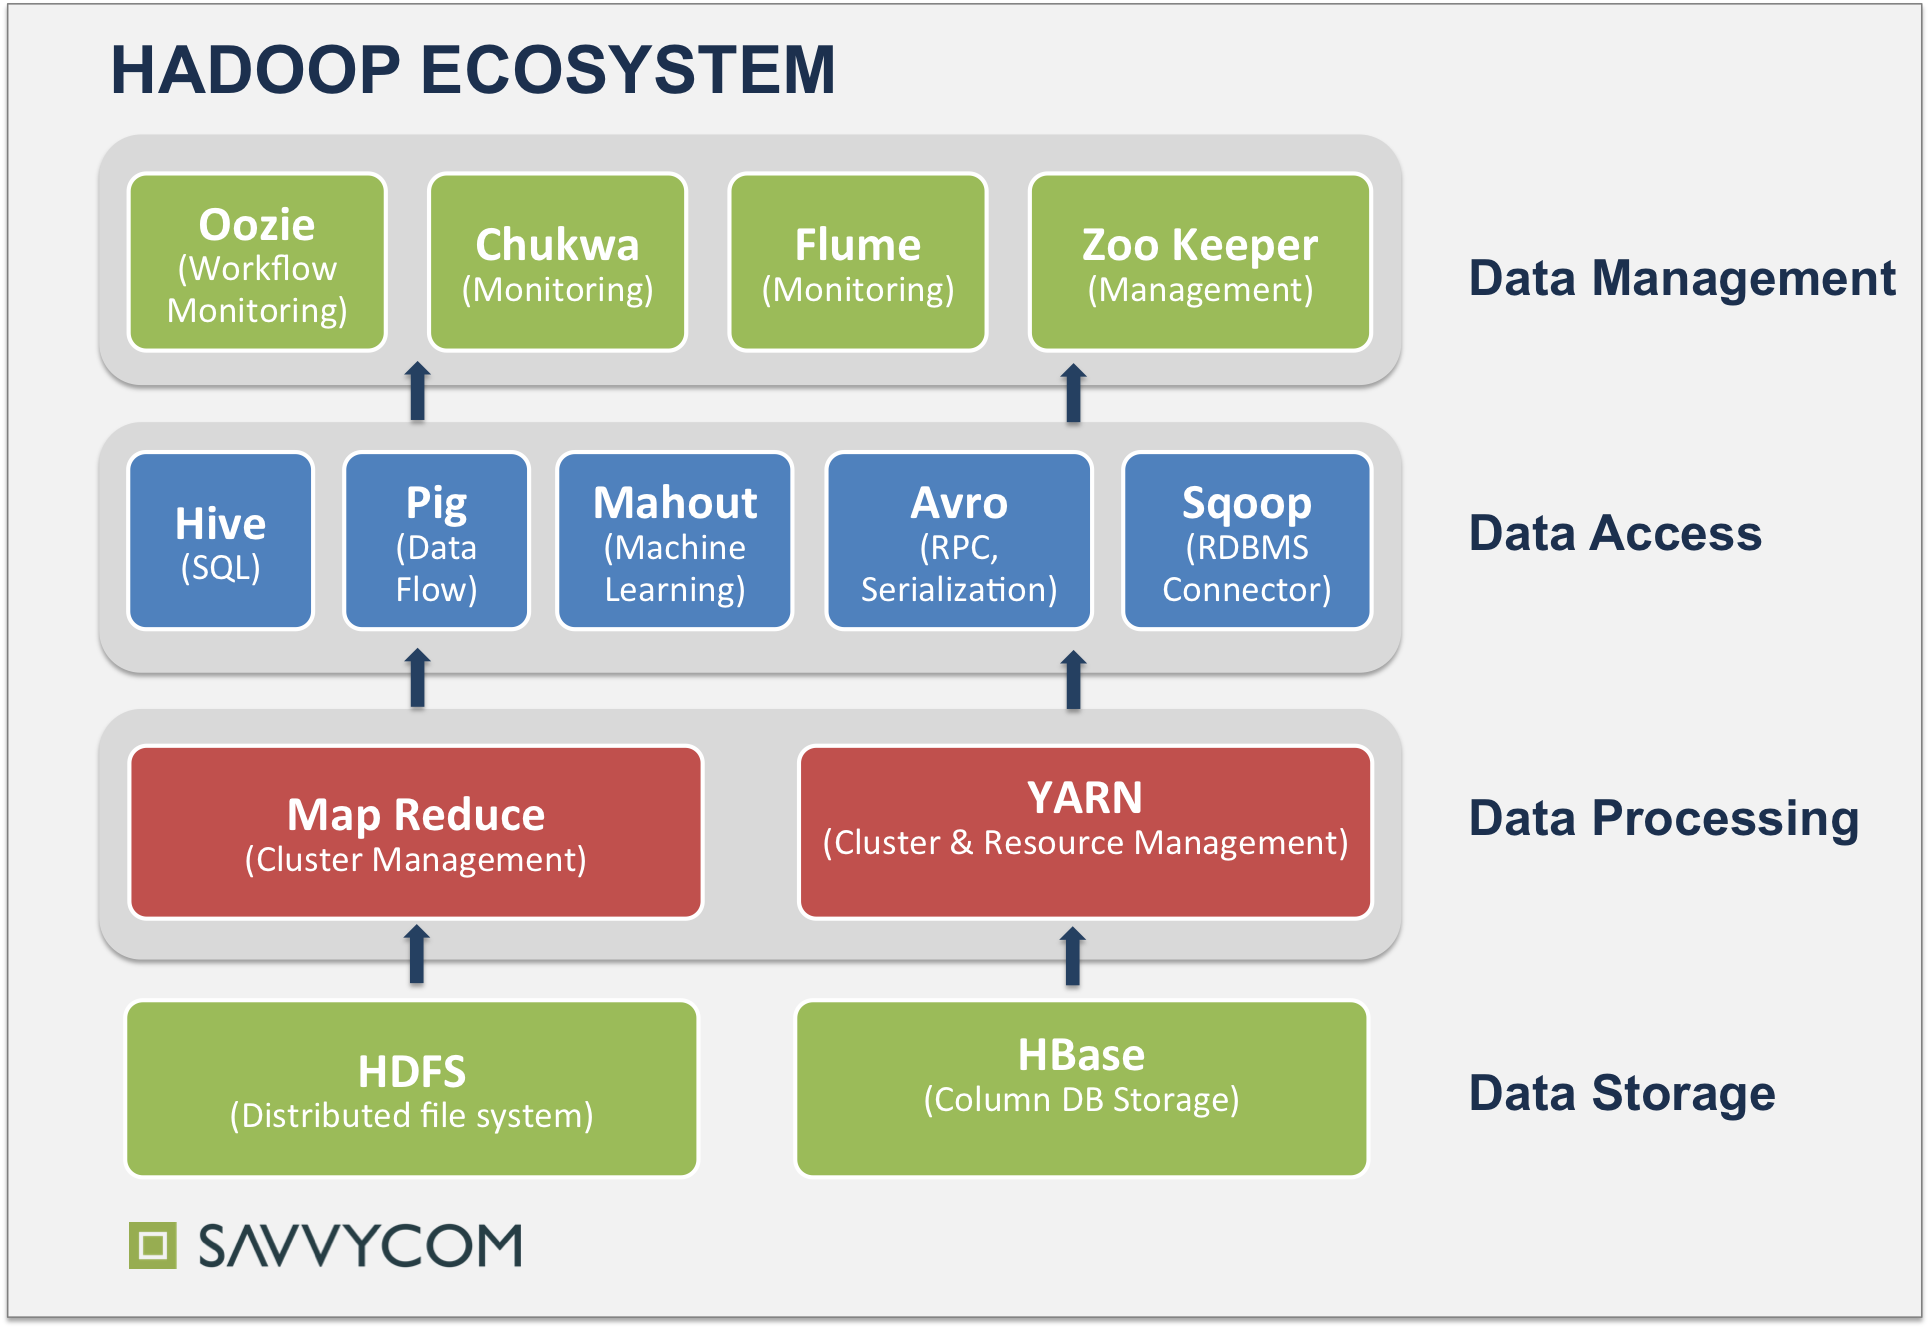
\includegraphics[width=0.60\linewidth]{content/images/HadoopEcosystem}\\
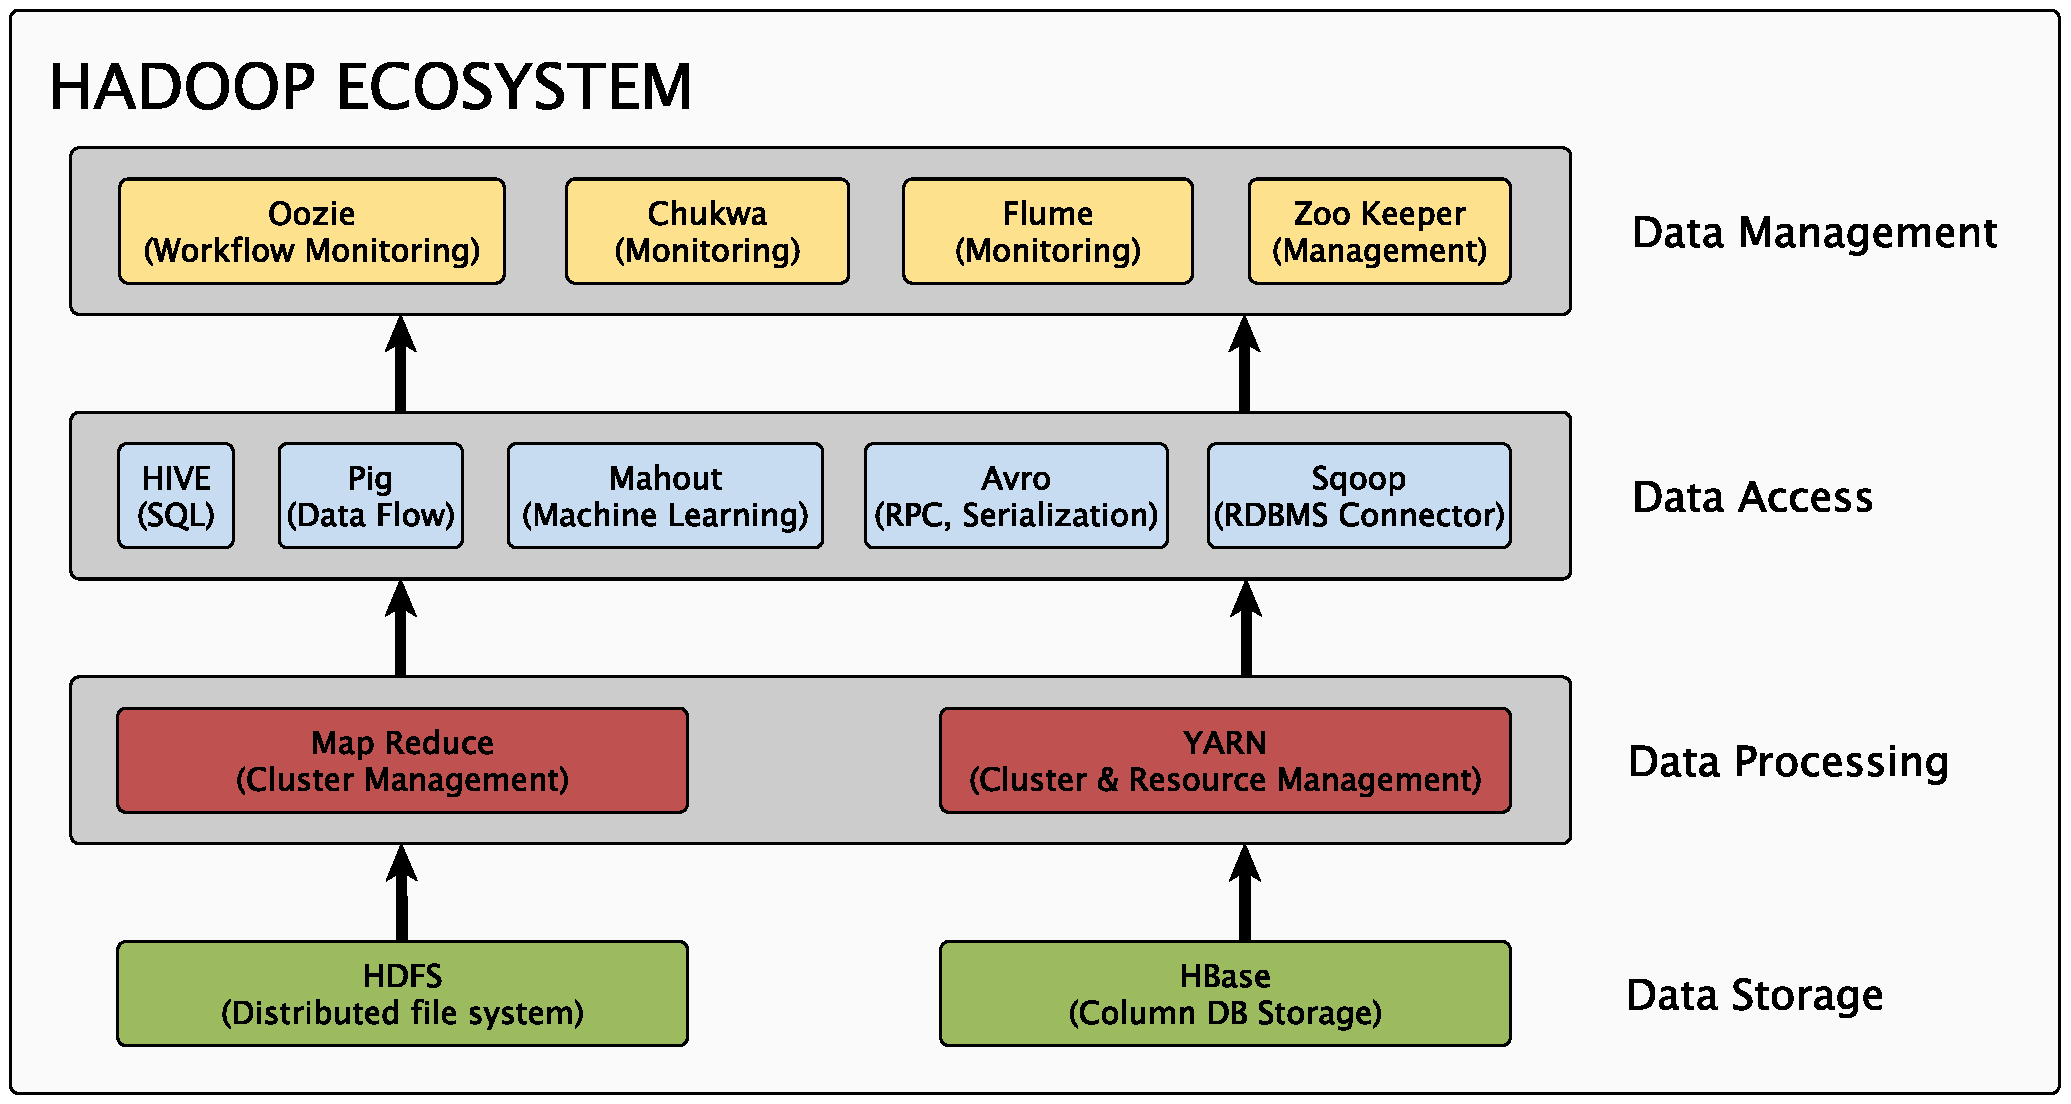
\includegraphics[width=0.70\linewidth]{content/drawings/hadoopEcosystem}

\caption{Hadoop Ecosystem.}
\label{fig:ecosystem}
\end{figure}

Built upon simple programming models, Hadoop can be scaled from single nodes to thousands of machines and runs on low-cost commodity hardware which is usually more vulnerable for failures than expensive, specialized hardware. To guarantee a highly-available service, the framework is designed to automatically detect and handle such failures.\\

What makes Hadoop different from traditional parallelism frameworks is its solution to the annoying I/O bottleneck typically arising in big data computations. Rather than bringing the data to the computing node, it brings the computation to the data. The fundaments of Apache Hadoop basically consists of the storage part \ac{HDFS} and the processing part MapReduce, which are in the focus of this paper.

\subsection{Hadoop Distributed File System (HDFS)}
The storage part, \ac{HDFS}, is a highly fault-tolerant filesystem designed to run on low-cost hardware which is inspired by the \ac{GFS}\cite{GFS}. \ac{HDFS} provides high-throughput access to application data and is tuned to support very large files. The files are split into large blocks (\eg 64~MB), replicated for reliability and distributed across various nodes in a cluster as illustrated in \Cref{fig:HDFS}.

\begin{figure}[ht]
\centering
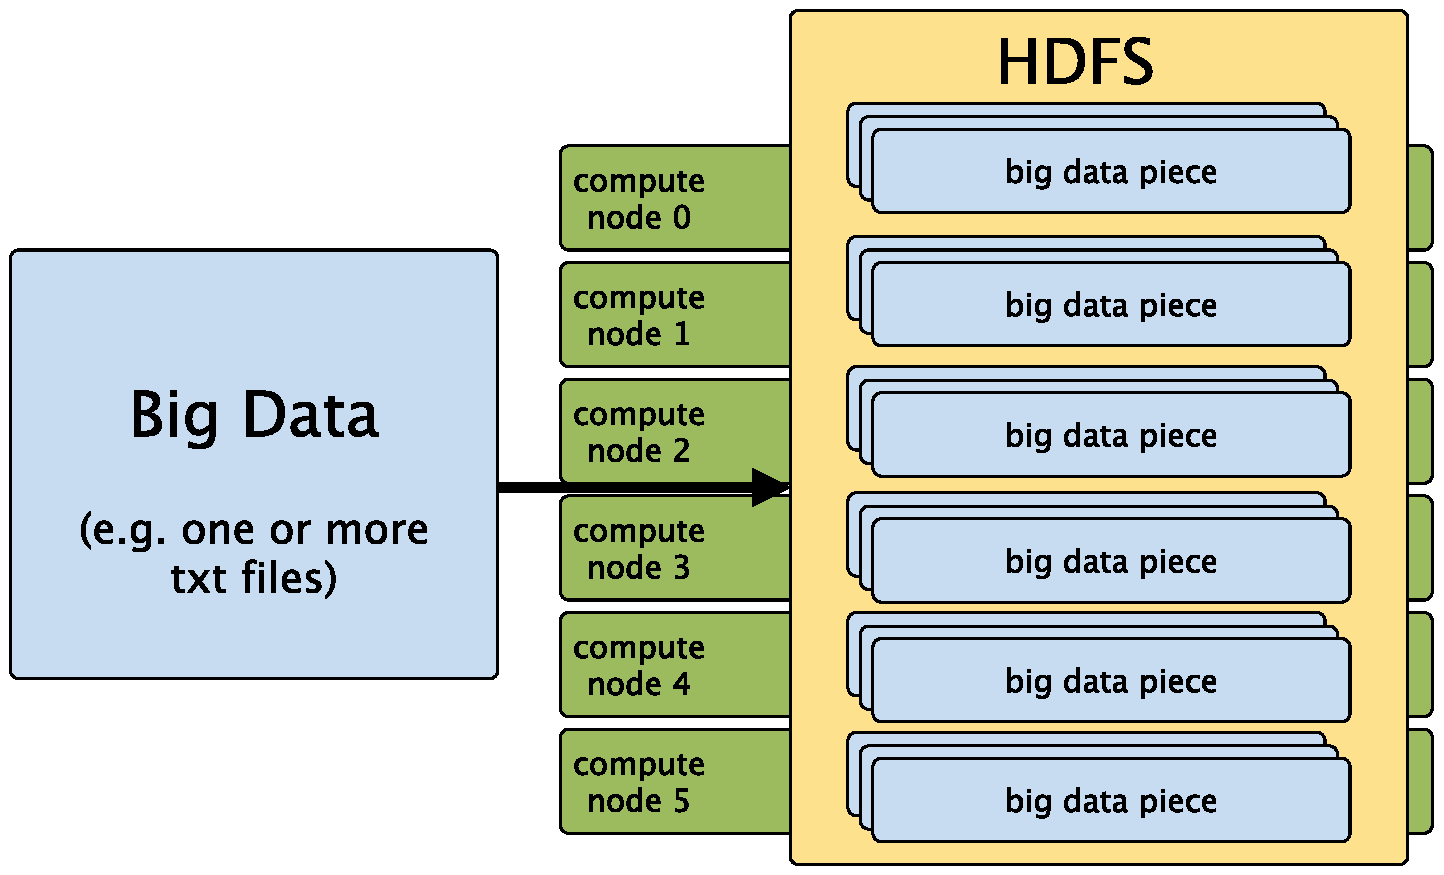
\includegraphics[width=0.50\linewidth]{content/drawings/BigDataDistribution}
\caption{File distribution across multiple physical compute nodes.}
\footnotesize 
\label{fig:HDFS}
\end{figure}
Typical file manipulation commands as e.g. \texttt{ls, mkdir, rm, mv, cp, cat, tail, chmod, ...} can be used to interact with files, while \ac{HDFS} takes care of recombining the data appropriately~\cite{lockwood}. These commands can be run via the Hadoop command  \texttt{hadoop dfs [GENERIC\_OPTIONS] [COMMAND\_OPTIONS]}.

\begin{tabular}[t]{ll}
Example & \texttt{hdfs dfs -ls /user/isresearch/}\\
 & \texttt{hdfs dfs -put ./1017\_01\_M\_08\_E\_20090331.csv /user/isresearch/}\\
\end{tabular}
\vspace{0.1cm}


\subsection{Hadoop MapReduce}
The processing part, Hadoop MapReduce, is an implementation of Googles MapReduce programming model~\cite{googleMapReduce} and is  composed of three phases:
\begin{description}
\item[Map()] In the first phase, each worker node applies the \emph{Map()} function to it's local part of the data. The data can be filtered and sorted in any desired form and will eventually be converted into zero or more key-value pairs.

\item[Shuffle()] In the second phase, the results from the previous \emph{Map()} phase are grouped according to their given key and stored back into the \ac{HDFS}. The Filesystem takes care of the redistribution of the intermediate results, such that all data of one key is located on the same physical node.

\item[Reduce()] In the last phase the worker nodes apply the \emph{Reduce()} function on each group of intermediate results individually and in parallel. The \emph{Reduce()} function performs a summary operation, such as counting the number of respective data points.
\end{description}

In contrast to traditional parallelism models, MapReduce performs the computation where the data resides, rather than transferring the data to the computation. As such, it avoids the previously mentioned I/O bottleneck, which arises from limited bandwidth and transportation cost induced by huge data files. Note that the individual phases must be complete before a succeeding phase can start. The typical MapReduce workflow is illustrated in \Cref{fig:mapreduceWorkflow}.

\begin{figure}[ht]
\centering
%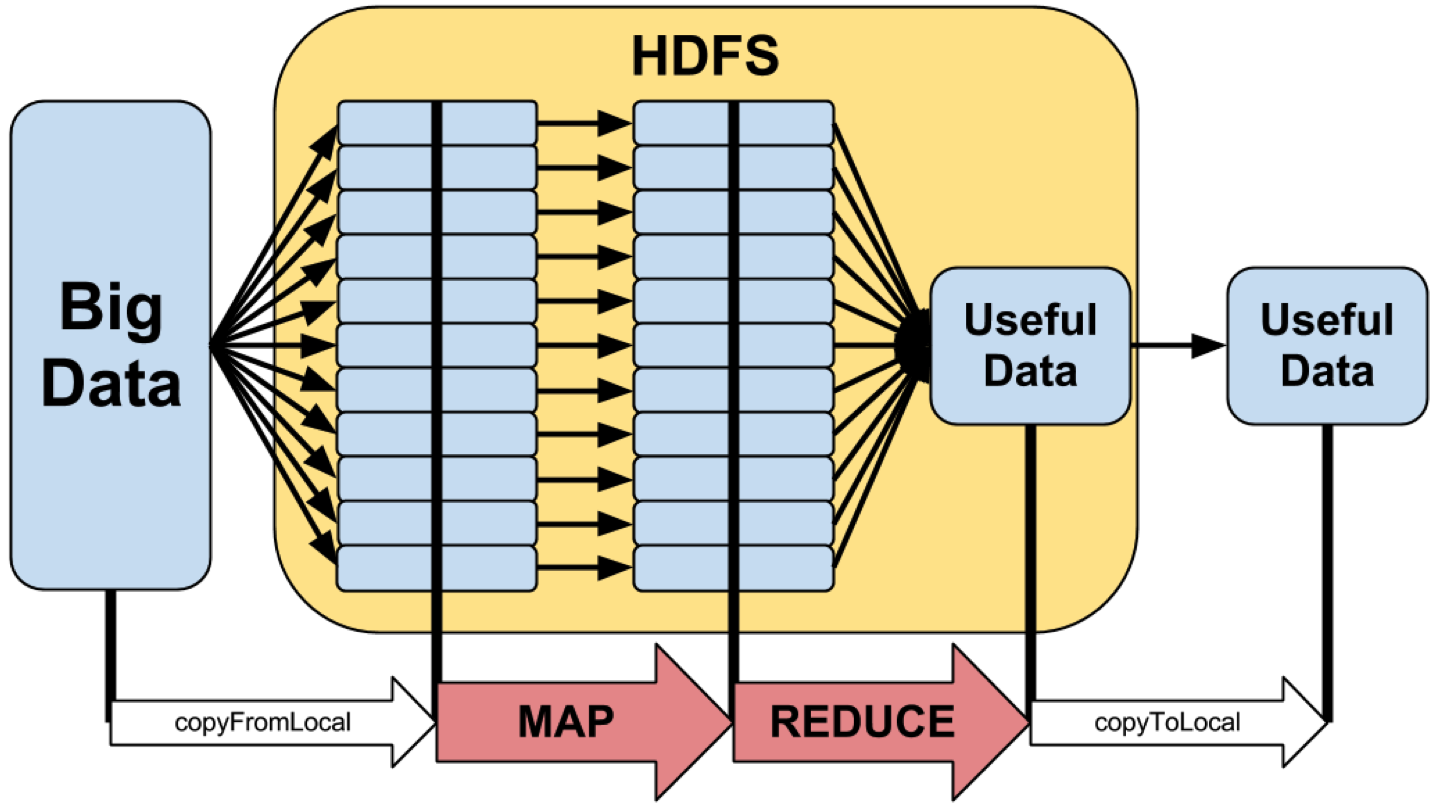
\includegraphics[width=0.60\linewidth]{content/images/mapreduce-workflow}\\
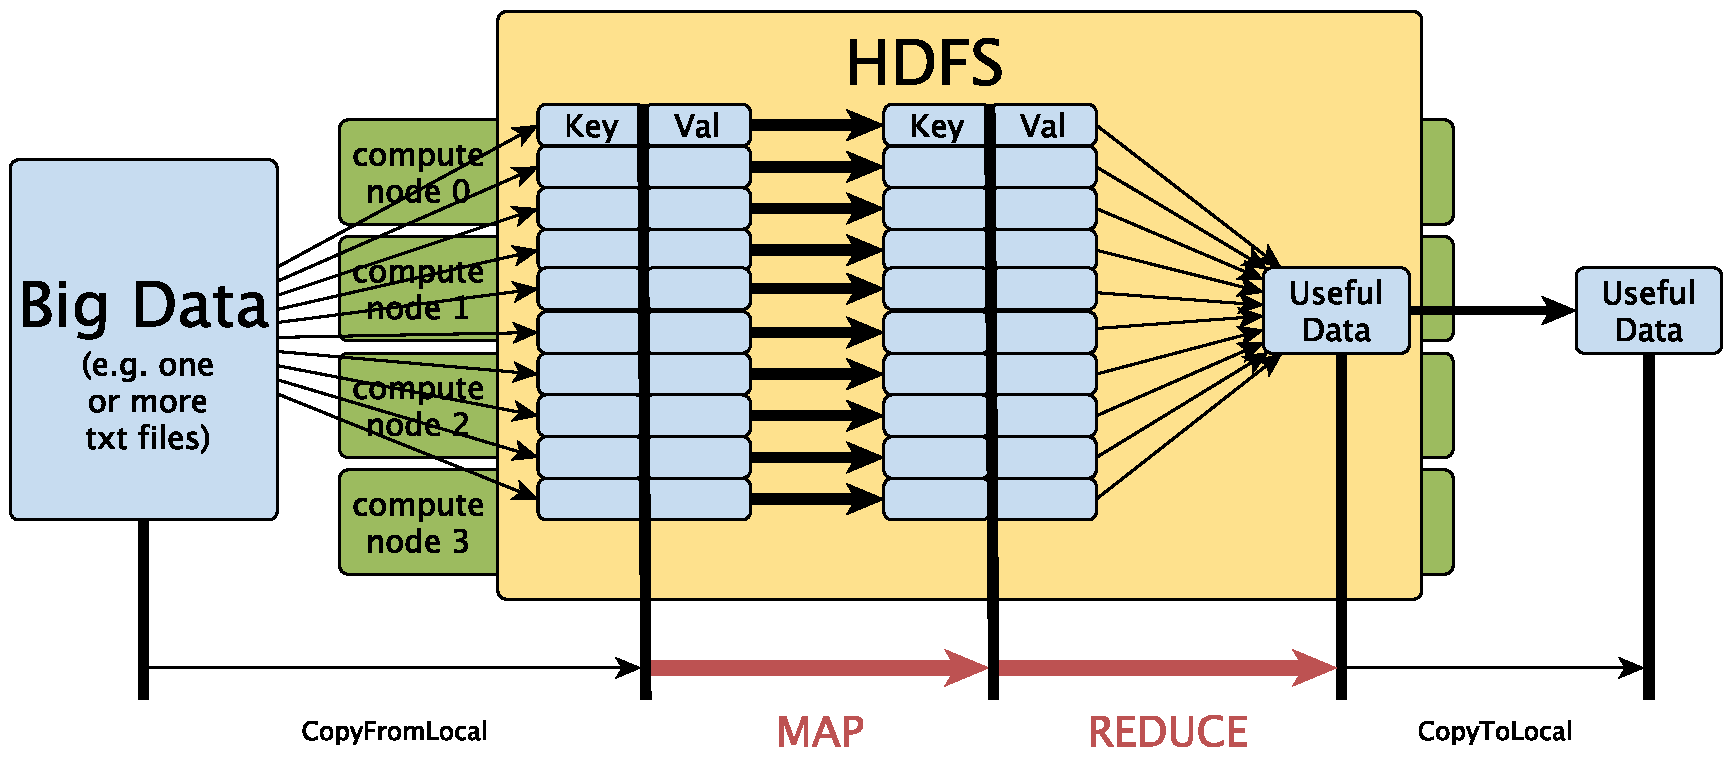
\includegraphics[width=0.70\linewidth]{content/drawings/MapReduceWorkflow}

\caption{MapReduce Workflow.}
\footnotesize 
\label{fig:mapreduceWorkflow}
\end{figure}


\subsubsection{Hadoop Streaming}
Hadoop Streaming~\cite{HadoopStreaming} is a generic API which comes with Hadoop. It allows Map and Reduce functions to be written in any language. Both functions read their respective input from stdin (line by line) and pass their output to stdout. The corresponding streaming format is shown in \Cref{lst:streaming}. The first part of each line until a delimiter (default: tab character) serves as the \emph{key}, while the rest of the line will be the \emph{value}. The output is always sorted by key.

\begin{lstlisting}[breaklines=true, caption=Default Hadoop Streaming format., escapechar=|, label={lst:streaming}]
key1 \t value1 \n
key2 \t value2 \n
key3 \t value3 \n
\end{lstlisting}


\chapter{Utilizing Hadoop from within R}
\label{chap:integration}
When analyzing big data, the capabilities of R and Hadoop fit together very well and should ideally be united. In the following, this paper describes how to utilize Hadoop from within the statistical software "R". 

\section{RHadoop}
The open source RHadoop project~\cite{rhadoop}, sponsored by Revolution Analytics, aims to give R programmers powerful tools to analyze data stored in Hadoop. RHadoop is a collection of five R packages as listed in \Cref{tab:rhadoop}.

\begin{table}
\begin{tabularx}{\textwidth{}}{|l|X|}\hline
rhdfs & This package provides basic connectivity to the Hadoop Distributed File System. R programmers can browse, read, write, and modify files stored in HDFS from within R. Install this package only on the node that will run the R client.\\\hline
rhbase & This package provides basic connectivity to the HBASE distributed database, using the Thrift server. R programmers can browse, read, write, and modify tables stored in HBASE, Hadoops distributed, scalable big data store database~\cite{HBase}. Install this package only on the node that will run the R client.\\\hline
plyrmr & This package enables the R user to perform common data manipulation operations, as found in popular packages such as plyr and reshape2, on very large data sets stored on Hadoop. Like rmr, it relies on Hadoop MapReduce to perform its tasks, but it provides a familiar plyr-like interface while hiding many of the MapReduce details. Install this package only every node in the cluster.\\\hline
rmr2 & A package that allows R developer to perform statistical analysis in R via Hadoop MapReduce functionality on a Hadoop cluster. Install this package on every node in the cluster.\\\hline
ravro & A package that adds the ability to read and write avro files from local and HDFS file system and adds an avro input format for rmr2. Install this package only on the node that will run the R client.\\\hline
  \end{tabularx}
\caption{RHadoop is a colletion of five R packages~\cite{rhadoop}.}
\label{tab:rhadoop}
\end{table}

The focus of this paper lies on the RHadoop packages \emph{rhdfs} and \emph{rmr2}, which allow R programmers to access the \ac{HDFS} and to perform statistical analysis in R via Hadoop MapReduce functionality on a Hadoop cluster. Detailed install instructions can be found on the projects website~\cite{rhadoop}.



\section{rhdfs}
Once \emph{rhdfs} is installed and the package is loaded, R programmers can browse, read, write and modify files stored in \ac{HDFS}. Amongst others the package offers functions for file manipulation (\texttt{hdfs.delete, hdfs.put, hdfs.get, \ldots{})}, read/write (\texttt{hdfs.file, hdfs.write, hdfs.seek, \ldots{}}) and utility (\texttt{hdfs.ls, hdfs.file.info, \ldots{}}). \\

As a prerequisite the environment variable HADOOP\_CMD must point to the full path of the \emph{hadoop} binary and the package must be initialized via \lstinline!hdfs.init()!. The corresponding code to define an environment variable, load the rhdfs library and initialize its functionality is shown in \Cref{lst:rhdfsInit}.

\begin{lstlisting}[breaklines=true, caption=Initialization of rhdfs., escapechar=|, label={lst:rhdfsInit}]
Sys.setenv(HADOOP_CMD="/usr/local/hadoop/bin/hadoop")
library(rhdfs)
hdfs.init()
\end{lstlisting}


\Cref{lst:RObjSerialization} shows exemplary how any R object can be serialized to HDFS. \Cref{line:writeFile} establishes a write connection (\lstinline!"w"!) to a, possibly not yet existing, file called \lstinline!"my_smart_unique_name"!. The R object \lstinline!model! is serialized and written into this file in \Cref{line:writeFile}. Finally the connection to that file must be closed.
\begin{lstlisting}[breaklines=true, caption=Serialization of an exemplary R object~\cite{rhadoop}., escapechar=|, label={lst:RObjSerialization}]
model <- lm(...)
modelfilename <- "my_smart_unique_name"
modelfile <- hdfs.file(modelfilename, "w")|\label{line:createFile}|
hdfs.write(model, modelfile)|\label{line:writeFile}|
hdfs.close(modelfile)
\end{lstlisting}

In contrast \Cref{lst:RObjDeserialization} shows the deserialization of an HDFS file to a R object. Here, a read connection (\lstinline!"r"!) to the desired \ac{HDFS} file is established to load its content into the R environment. Subsequently the retrieved content must be unserialized (\Cref{line:unserialize}) and again the connection must be closed.
\begin{lstlisting}[breaklines=true, caption=Deserialization of an exemplary R object~\cite{rhadoop}., escapechar=|, label={lst:RObjDeserialization}]
modelfile = hdfs.file(modelfilename, "r")
m <- hdfs.read(modelfile)
model <- unserialize(m)|\label{line:unserialize}|
hdfs.close(modelfile)
\end{lstlisting}



\section{rmr2}\label{sec:rmr2}
With the help of \emph{rmr2} programmers can utilize the Hadoop MapReduce functionality from within R to perform statistical analysis on huge data sets on a parallel basis.\\

Similar as for \emph{rhdfs} it is necessary to set the environment variables HADOOP\_CMD and HADOOP\_STREAMING, the latter one pointing to the Hadoop Streaming Java\footnote{Apache Hadoop is implemented in Java} Library. An example initialization is show in \Cref{lst:rmr2Init}.
\begin{lstlisting}[breaklines=true, caption=Initialization of the rmr2 package., escapechar=|, label={lst:rmr2Init}]
Sys.setenv(HADOOP_CMD="/usr/local/hadoop/bin/hadoop")
Sys.setenv(HADOOP_STREAMING
              ="/usr/local/hadoop/share/hadoop/tools/lib/hadoop-streaming-2.4.1.jar")
library(rmr2)
rmr.options(backend="hadoop")|\label{line:backend}|
\end{lstlisting}

Via \lstinline!rmr.options()! it is possible to switch between the distributed Hadoop backend (see \Cref{line:backend}) and a non-distributed local backend. With \lstinline!backend="local"! rmr2 jobs run single threaded on the local interpreter which helps a lot when debugging. By default, all nodes will receive a copy of the global R environment, \ie they can read previously initialized variables. To reduce transfer costs the option \lstinline!rmr.options(exclude.objects=NULL)! can exclude certain objects from this practice.\\

The most important function provided by rmr2 is \lstinline!mapreduce()!. \Cref{lst:structMapReduce} shows the functions signature as documented in the R documentation. The function defines and runs a MapReduce job on a given input (either an object or a valid path string). Various parameters allow an individual fine tuning of the MapReduce job. \Eg:

\begin{description}
\item[input] Paths to the input folder(s) or the return value of another mapreduce or a \lstinline!to.dfs!\footnote{\texttt{to.dfs()} and \texttt{from.dfs()} allow to move data from RAM to HDFS and back.  \cite[R help of rmr2,][]{rhadoop}} call.
\item[input.format] \lstinline!= make.input.format("csv", sep = ";")! defines the format and structure of the input file(s).
\item[output] defines the destination path in the HDFS. If absent, \lstinline!mapreduce()! returns a \texttt{big.data.object}\footnote{A \texttt{big.data.object} references a data set stored in the HDFS. As such even huge data sets that exceed the nodes memory can be manipulated by other rhadoop functions. \cite[R help of rmr2,][]{rhadoop}}, otherwise it returns the \ac{HDFS} filepath.
\item[map] an R function of two arguments specifying the map phase. It either returns \lstinline!NULL! or a collection of key-value pairs.
\item[reduce] an R function which takes as an input the key-value pairs generated by the preceding map phase grouped by key.
\end{description}

\begin{lstlisting}[breaklines=true, caption=function signature of \lstinline!mapreduce()! as described in the rmr2 help (\lstinline!?mapreduce!)., escapechar=|, label={lst:structMapReduce}]
mapreduce(
  input,
  output = NULL,
  map = to.map(identity),
  reduce = NULL,
  vectorized.reduce = FALSE,
  combine = NULL,
  in.memory.combine = FALSE,
  input.format = "native",
  output.format = "native",
  backend.parameters = list(),
  verbose = TRUE) 
\end{lstlisting}


\section{Word Count Example}\label{chap:helloWorld}
\Cref{lst:helloWorld} shows a simple "Hello World!" example for a MapReduce job~\cite{usingRAndHadoop}. The jobs intend is to return the number of word occurrences within a given input text file. The input file \texttt{loremipsum.txt} contains 100 words of dummy text and as such \lstinline!input.format! is simply \lstinline!"text"!.

Our map function, defined in \Cref{line:mapFunc}, reads the input line by line and splits each line into individual words. Using the individual words as key and integer one as a counter variable, it produces corresponding key-value pairs. In the next phase, the mapper function, defined in \Cref{line:redFunc}, receives the grouped key-values and simply outputs the sum over all counter 'ones' for each key. In \Cref{line:fromDFS} the final result is moved into the R environment and can be viewed or further processed.

\begin{lstlisting}[breaklines=true, caption=Hello World example for MapReduce~\cite{usingRAndHadoop}., escapechar=|, label={lst:helloWorld}]
library(rmr2)
rmr.options(backend = "local")
data <- mapreduce(input = "loremipsum.txt", 
                  input.format = "text",
                  map = function(.,lines){|\label{line:mapFunc}|
                    keyval(key = unlist(strsplit(lines, split = " ")),
                           val = 1) },
                  reduce = function(word, counts){|\label{line:redFunc}|
                    keyval(key = word,
                           val = sum(counts)) }
)
result = from.dfs(data)|\label{line:fromDFS}|
result$key
 [1] "Lorem"      "ipsum"      "dolor"      "sit"        "amet,"      "consetetur"  ...
result$val
 [1] 4 4 4 4 2 2 2 2 4 4 2 2 2 2 2 2 8 2 2 2 2 2 2 2 2 2 2 2 2 2 2 2 2 2 2 2 2 2 2 2 2
\end{lstlisting}

\chapter{Real World Example: Stock Exchange Data}
\label{chap:example}
This chapter is about a concrete, real world example. The seminars secondary task was to analyze stock exchange data to find out how fast automated traders respond to published ad~hoc messages. The complete code for this example can be found online at \cite{GitHubAxelPerschmann} and is split into several R scripts:\\

\begin{tabular}[t]{ll}
0\_helloWorld.R & Initial hello world example (\Cref{chap:helloWorld}) \\
1\_dataToHDFS.R & Unzip and transfer stock data into the \ac{HDFS} (\Cref{chap:transferHDFS})\\
2\_parse\_adHocXML.R & Parsing of available adhoc messages (\Cref{chap:adHocMessages})\\
3a\_hadoop\_checkTimeZone.R & Little experiment to verify correct timezone (\Cref{chap:timeZoneCheck})\\
3\_hadoop.R & Defining and running the MapReduce job (\Cref{chap:MapReduceJob}) \\
4\_evaluation.R & Evaluation and plotting of results (\Cref{chap:evaluation})\\
  \end{tabular}

\section{Input Data}
\subsection{Stock exchange data from the Deutsche B\"orse}
The analyzation is based on 166 files (200+ GB) of tick data, obtained from the universities exclusive access to the Deutsche B\"orse. 
Exact to the hundredth of a second they contain millions of transitions, each encoded as follows:

\begin{tabular}[t]{ll}
\texttt{WKN, ISIN} & Instrument identifiers\\
\texttt{INSTRUMENT\_NAME} & Instrument name\\
\texttt{TIMESTAMP, HSEC} & Exact timestamp\\
\texttt{PRICE} & Current price\\
\texttt{UNITS} & Number of units\\
\texttt{BID\_ASK\_FLAG} & BID or ASK\\
  \end{tabular}\\
  
An excerpt from one of the files is shown in \Cref{lst:tickData}.

\begin{lstlisting}[breaklines=true, caption=Excerpt from monthly\_bba\_aa\_20090331.csv., escapechar=|, label={lst:tickData}]
                                                                                   BID_ASK
WKN   ;ISIN        ;INSTRUMENT_NAME          ;TIMESTAMP          ;HSEC;PRICE;UNITS;_FLAG
940602;NL0000009538;KON.PHILIPS.ELECT.  EO-20;2009-03-02 12:04:00; 92 ;12.06; 8572;A
843002;DE0008430026;MUENCH.RUECKVERS.VNA O.N.;2009-03-02 12:04:00; 94 ;92.34;   46;A
840400;DE0008404005;ALLIANZ SE VNA O.N.      ;2009-03-02 12:04:00; 94 ;50.89;   90;A
LYX0A0;FR0010344986;LYXOR ETF DJ ST. 600 RET.;2009-03-02 12:04:00; 94 ;18.29;10000;B
\end{lstlisting}
\label{chap:timeZoneCheck}
In the early phase of testing the subsequent MapReduce job on only one of these 166 input files (monthly\_bba\_aa\_20090331.csv) very little trade activity could be observed. As the given timestamps do not include a timezone definition a little experiment was performed to exclude the case of a miss interpretation. \emph{3a\_hadoop\_checkTimeZone.R} analyzes how trade activity is distributed in terms of daytime. \Cref{fig:timezone} clearly depicts that there is no offset in between observed trades and the trading hours of Xetra which are between 8.50 a.m. CET and 5.30 p.m. CET~\cite{xetra}.

\begin{figure}[ht!]
\centering
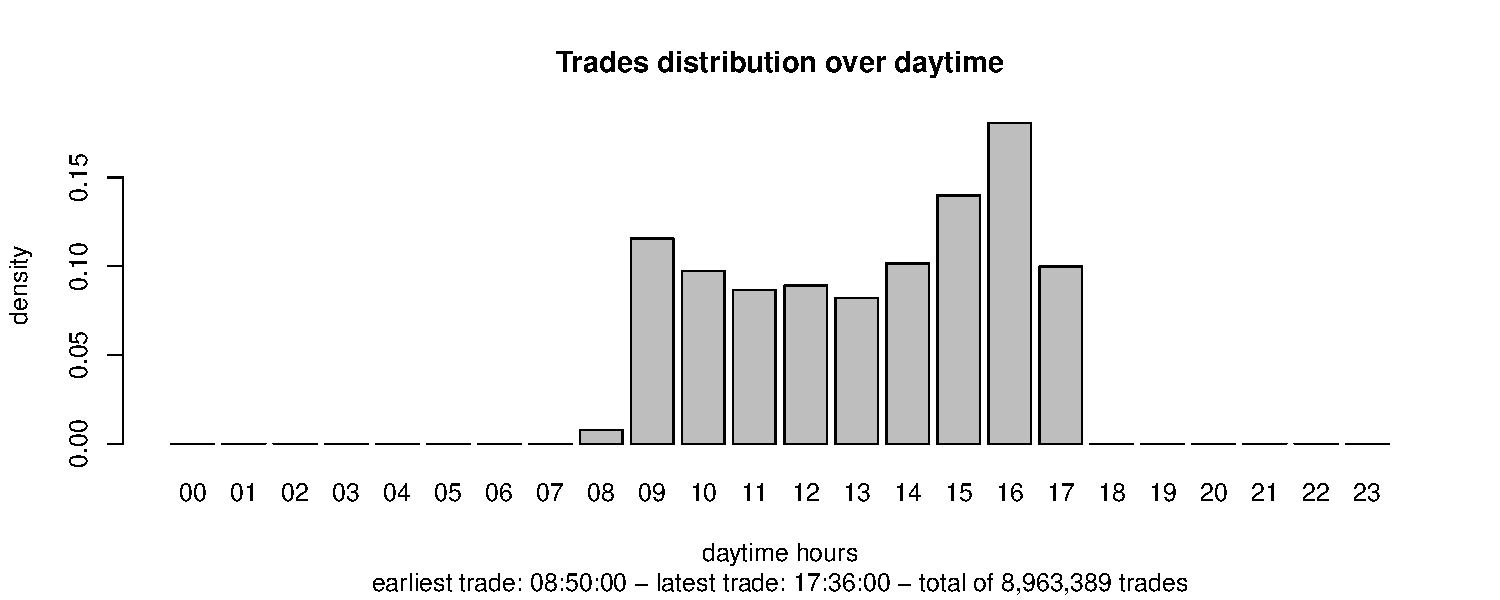
\includegraphics[width=0.7\linewidth]{content/pdf/trade_distribution_new} %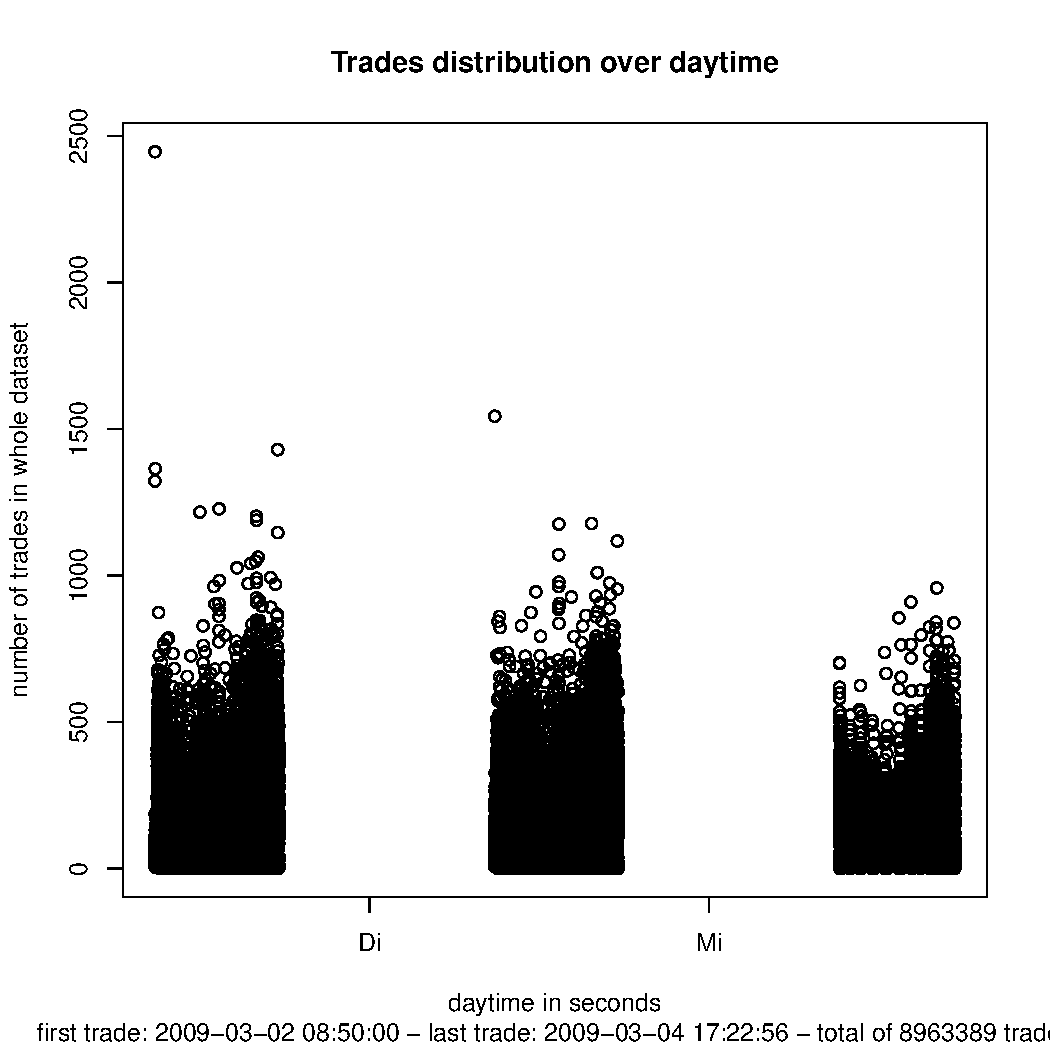
\includegraphics[width=0.35\linewidth]{content/pdf/trade_distribution_date}
\caption{Trade distribution within monthly\_bba\_aa\_20090331.csv.}
\label{fig:timezone}
\end{figure}

\subsection*{Transfer into HDFS}\label{chap:transferHDFS}
All 166 files came as compressed zip files. \Cref{lst:dataToHDFS} shows how these files were unzipped and transferred into the \ac{HDFS}.�\\

As a first step a new directory on the \ac{HDFS} was created using the \lstinline!hdfs.mkdir! command (\Cref{line:mkdir}). Then a for-loop, iterating over all 166 .zip files found in the local directory \lstinline!DeutscheBoerse/!, unzips the contained csv files into a temporary folder \lstinline!DeutscheBoerse/tmp/! and finally transfers the data into the \ac{HDFS} using the \lstinline!hdfs.put! command (\Cref{line:put}). Because the zipped files consume only 260~MB while the unzipped versions take 1.35~GB the latter ones were immediately discarded after they had been transferred to the \ac{HDFS}.

\begin{lstlisting}[breaklines=true, caption=1\_dataToHDFS.R., escapechar=|, label={lst:dataToHDFS}]
Sys.setenv(HADOOP_CMD="/usr/local/hadoop/bin/hadoop")
library(rhdfs)
hdfs.init()

setwd("DeutscheBoerse")
input.names = list.files(path = ".", pattern=".*zip")

# create new directory on HDFS
hdfs.mkdir("/user/isresearch/Data")|\label{line:mkdir}|

# push files to HDFS. Only necessary once!
for (name in input.names) {
  print(name)
  # unzip file and read name of extracted file
  unzip(name, exdir = "tmp/")
  source.name = list.files(path = "tmp")
  
  path.source = paste(getwd(), "/tmp/", source.name, sep="")
  path.dest = paste("/user/isresearch/Data/", source.name, sep="")
  # load to HDFS
  hdfs.put(src=path.source, dest=path.dest)|\label{line:put}|
  
  # do not keep large unzipped file
  unlink(paste(getwd(), "/tmp", sep=""), recursive=TRUE)
}
\end{lstlisting} 

\subsection*{Input format}\label{sec:inputdata}
As we want to process csv files, we have to specify the input format of our mapreduce job, as briefly mentioned in \Cref{sec:rmr2}. In \Cref{lst:inputFormat} we define the csv file separator, the column names and that we do not want strings to be interpreted as factors. Unfortunately \lstinline!make.input.format()! does not come with a parameter like \lstinline!header=TRUE!, such that we have to consider this in our map function where we must discard the headerline.

\begin{lstlisting}[breaklines=true, caption=Input format., escapechar=|, label={lst:inputFormat}]
inputformat <- make.input.format("csv", sep = ";", stringsAsFactors = FALSE,
                              col.names=c("WKN", "ISIN", "INSTRUMENT_NAME", "TIMESTAMP", 
                                           "HSEC", "PRICE", "UNITS", "BID_ASK_FLAG") )
rmr.options(backend="hadoop")
files = hdfs.ls("Data")[,6]         # all filenames in dir /user/isresearch/Data/
files = files[grep(".*csv", files)] # filter for csv files only
\end{lstlisting}


\subsection{Ad~hoc messages}\label{chap:adHocMessages}
An additional collection of seven xml-files ($\approx170$~MB in total) contain individual ad~hoc messages including their respective date and time of publication. The seminars task included the extraction of corresponding (\texttt{TIMESTAMP, ISIN})-pairs using regular expressions. Due to the relatively small size of these xml files this sub task was solved entirely on the local machine and the results stored into a csv file.\\

To make the xml parsing a little complicated, the structure and content of the files vary. In some files the \texttt{ISIN} can directly be read from a field called \lstinline!"isin"!, whereas other files are lacking this field and therefore enforce the use of a regular expression search over the whole message text. Furthermore some messages include only dates and text and do not mention any \texttt{ISIN}. Those messages were discarded and ignored by \emph{2\_parse\_adHocXML.R}. The final version of the regular expression, utilized to extract an \texttt{ISIN} from the raw ad~hoc message text, is shown in \Cref{lst:regEx}.
\begin{lstlisting}[breaklines=true, caption=Regular Expression to extract an ISIN from text., escapechar=$, label={lst:regEx}]
expr = paste("(XS|AD|AE|AF|AG|AI|AL|AM|AO|AQ|AR|AS|AT|AU|AW|AX|AZ|BA|BB|BD|",
               "BE|BF|BG|BH|BI|BJ|BL|BM|BN|BO|BQ|BR|BS|BT|BV|BW|BY|BZ|CA|CC|",
               "CD|CF|CG|CH|CI|CK|CL|CM|CN|CO|CR|CU|CV|CW|CX|CY|CZ|DE|DJ|DK|",
               "DM|DO|DZ|EC|EE|EG|EH|ER|ES|ET|FI|FJ|FK|FM|FO|FR|GA|GB|GD|GE|",
               "GF|GG|GH|GI|GL|GM|GN|GP|GQ|GR|GS|GT|GU|GW|GY|HK|HM|HN|HR|HT|",
               "HU|ID|IE|IL|IM|^IN|IO|IQ|IR|IS|IT|JE|JM|JO|JP|KE|KG|KH|KI|KM|",
               "KN|KP|KR|KW|KY|KZ|LA|LB|LC|LI|LK|LR|LS|LT|LU|LV|LY|MA|MC|MD|",
               "ME|MF|MG|MH|MK|ML|MM|MN|MO|MP|MQ|MR|MS|MT|MU|MV|MW|MX|MY|MZ|",
               "NA|NC|NE|NF|NG|NI|NL|NO|NP|NR|NU|NZ|OM|PA|PE|PF|PG|PH|PK|PL|",
               "PM|PN|PR|PS|PT|PW|PY|QA|RE|RO|RS|RU|RW|SA|SB|SC|SD|SE|SG|SH|",
               "SI|SJ|SK|SL|SM|SN|SO|SR|SS|ST|SV|SX|SY|SZ|TC|TD|TF|TG|TH|TJ|",
               "TK|TL|TM|TN|TO|TR|TT|TV|TW|TZ|UA|UG|UM|US|UY|UZ|VA|VC|VE|VG|",
               "VI|VN|VU|WF|WS|XF|YE|YT|ZA|ZM|ZW)([\\s]?)",
               "(?=.{0,8}[0-9]+)([0-9A-Z]{9}[0-9]?)",
               "(?![0-9]{1})",
               sep="")
  # 2 characters:   country
  # 9 alphanumeric: NSIN
  # 1 number:       optional checksum
\end{lstlisting}

The resulting list of 33\,617 distinct (\texttt{TIMESTAMP, ISIN})-pairs \lstinline!ev! was ordered by \texttt{ISIN} and \texttt{TIMESTAMP} successively and eventually stored into a csv file as shown in \Cref{lst:eventsToCSV}.

\begin{lstlisting}[breaklines=true, caption=Sorting and storage of events.csv., escapechar=$, label={lst:eventsToCSV}]
ev = unique(data.frame(events))

# sort stuff
library(dplyr)
ev = arrange(ev, isin, date)

write.csv(ev, file="events.csv", row.names=FALSE)
\end{lstlisting}

\section{MapReduce Job}\label{chap:MapReduceJob}
Before defining and running the MapReduce job in \Cref{lst:isin.list}, we ensure the previously generated list \lstinline!ev! is available in the global R environment such that our reduce function can access the ad~hoc message dates. We further generate a smaller \lstinline!isin.list! which aggregates all distinct \texttt{ISIN}s contained in \lstinline!ev!, such that our map function can discard data points not belonging to any of these \texttt{ISIN}s.

\begin{lstlisting}[breaklines=true, caption=ev and isin.list are loaded into the global R environment., escapechar=|, label={lst:isin.list}]
# load isin_set
ev = read.csv("events.csv", sep=",", as.is=TRUE, col.names=c("date", "ISIN"))
isin.list = as.character(unique(ev[,2]))
\end{lstlisting}

\subsection{Map() function}\label{sec:mapper}
Multiple, parallel running instances of the Map() function as shown in \Cref{lst:mapFunction} transfer small junks of the whole input into (key, value)-pairs.\\

Each instance receives it's part of the input as value matrix \lstinline!v!, where the different values are accessible by their respective column name (\eg \lstinline!v$PRICE!). The key vector \lstinline!k! is empty, except for the case of chaining multiple MapReduce jobs together.

\begin{lstlisting}[breaklines=true, caption=Map() function., escapechar=|, label={lst:mapFunction}]
map.ticks <- function(k, v) {
  # Skip header lines
  v = v[v$PRICE != "PRICE",]|\label{line:header}|
  v$PRICE = as.double(v$PRICE)|\label{line:double}|
  v = v[v$PRICE != 0.0, ] # erroneous values in data?!|\label{line:erroneous}|
  
  # only extract ISIN's when we have observed an AdHoc msg
  v = cbind(v, useful=v$ISIN %in% isin.list)|\label{line:useful}|
  v = v[v$useful == TRUE,]
  
  keyval(key=paste(v$ISIN, v$BID_ASK_FLAG, sep="_"),
         val=subset(v, select=c("TIMESTAMP", "PRICE")))|\label{line:subset}|
}
\end{lstlisting}

As mentioned in \Cref{sec:inputdata}, we need to filter out the header line. In \Cref{line:header} we discard all rows whose \lstinline!v$PRICE! contains the string \lstinline!"PRICE"! rather than a number. Once the header is gone, we can convert column \lstinline!v$PRICE! from character to double (\Cref{line:double}) and discard erroneous values (\Cref{line:erroneous}). A major reduction of the data is achieved in \Cref{line:useful}, where we check wether a data points \texttt{ISIN} is present in \lstinline!isin.list! (\lstinline!useful=TRUE!) or not (\lstinline!useful=FALSE!). Only useful values will be kept. Finally we define the key as a concatenation of \texttt{ISIN} and \texttt{BID\_ASK\_FLAG} (\eg \lstinline!"DE0007664039_A"!, \lstinline!"DK0010272632_B"!) and the value is further reduced to the columns of interest: \texttt{TIMESTAMP} and \texttt{PRICE}.


\subsection{Reduce() function}\label{sec:reducer}
After the map phase has finished, the ordered (key, value)-pairs are distributed across multiple, parallel running instances of the Reduce() function shown in \Cref{lst:redFunction}.

\begin{lstlisting}[breaklines=true, caption=Reduce() function., escapechar=|, label={lst:redFunction}]
red.ticks <- function(k, v) {
  v$TIMESTAMP = as.POSIXct(v$TIMESTAMP, "%Y-%m-%d %H:%M:%OS", tz="CET")
  v = v[order(v$TIMESTAMP),]
  
  adhocs = ev[ev$ISIN == unlist(strsplit(k, "_"))[1], 1]
  adhocs = as.POSIXct(adhocs, "%Y-%m-%d %H:%M:%OS", tz="CET")
  adhocs = adhocs[!is.na(adhocs)]
  
  # only keep adhoc dates which lay in the interval of available tick data
  adhocs.relevant = adhocs[adhocs > v$TIMESTAMP[1]]|\label{line:adHocFilter}|
  adhocs.relevant = adhocs.relevant[adhocs.relevant < tail(v$TIMESTAMP, n=1)]
  
  if (length(adhocs.relevant) > 0) {
    # compute price deltas for fixed intervals
    l = length(adhocs.relevant)
    offset.seconds = c(0, 1, 5, 10, 30, 60, 60*5, 60*10, 60*60)
    timestamps = matrix(rep(adhocs.relevant,length(offset.seconds)), nrow=l)
    offset = matrix(rep(offset.seconds, l), byrow=TRUE, nrow=l)
    timestamps.future = timestamps + offset
    
    fun = stepfun(v$TIMESTAMP, c(v$PRICE, tail(v$PRICE, n=1)), f=0, right=TRUE)|\label{line:stepFun}|
    
    # collect corresponding PRICE for each TIMESTAMP
    result = c()
    for (i in 1:l) {
      x = fun(timestamps.future[i,])
      result = rbind(result, x)
    }
    colnames(result) = paste("+", offset.seconds, "s", sep="")
    
    # calculate PRICE delta over time
    delta = result / result[,1]
    colnames(delta) = paste("s", offset.seconds, sep="")
    rownames(delta) = make.names(adhocs.relevant, unique=TRUE)
    
    keyval(key=cbind(isin=k, date=as.character(adhocs.relevant)), 
           val=delta)
  }
}\end{lstlisting}
After an initial character to POSIXct\footnote{\url{https://stat.ethz.ch/R-manual/R-devel/library/base/html/DateTimeClasses.html}, accessed: 17-June-2016} conversion and subsequent order-by-time command, we extract all ad~hoc timestamps belonging to the current \texttt{ISIN} from \lstinline!ev!. In \Cref{line:adHocFilter}f. we discard dates of ad~hoc messages that occurred outside the available tick data range. \\

For the remaining adhoc dates we check the stock price 1s, 5s, 10s, 30s, 60s, 5m, 10m and 1h after publication of the particular message and compute the respective deltas in percent. For this purpose, we convert the available stock data points into a step function (\Cref{line:stepFun}). Parameter \lstinline!f=0! disables interpolation between the given x values, such that the functions return value always corresponds to the last price observed before the queried time point.\\

The function finally returns the computed deltas for every applicable (\texttt{ISIN, ad~hoc})-pair.

\subsection{MapReduce job call}
The final call of the MapReduce job is shown \Cref{lst:mapReduceJob}. The variables \lstinline!files! and \lstinline!inputformat! were introduced in chapter \ref{sec:inputdata}, \lstinline!map.ticks! in \Cref{sec:mapper} and \lstinline!red.ticks! in \Cref{sec:reducer}.\\

The job's output will be stored into the \ac{HDFS} as a csv file while the function \lstinline!mapreduce()! returns the associated filepath. To further view or process the data in RStudio \lstinline!from.dfs()! loads the output into the R environment.

\begin{lstlisting}[breaklines=true, caption=Running the MapReduce job., escapechar=|, label={lst:mapReduceJob}]
library(rmr2)
rmr.options(backend="hadoop")

data<- mapreduce(input=files
                 ,input.format=inputformat
                 ,output="user/isresearch/output.csv"
                 ,output.format=make.output.format("csv", sep=";")
                 ,map = map.ticks
                 ,reduce = red.ticks
)
data.df = from.dfs(data, format=make.input.format("csv", sep=";"))
\end{lstlisting}

\section{Evaluation}\label{chap:evaluation}
Once the MapReduce job has finished successfully and the data is loaded into the R environment, we can finally generate some statistics. The examples task was to find out how fast automated traders respond to published ad~hoc messages. The evaluation code is available at \cite{GitHubAxelPerschmann}.\\

\Cref{fig:tradeActivity} shows the ratio of samples where an ad~hoc message was shortly after followed by a price fluctuation. In 58 of 8565 cases (0.7\%) a trade had happened within the first second after the publication, whereas after 1 minute the activity rate was already at 8.6\%. One hour after publication, 29.9\% off all examples where affected by a price fluctuation. The Figure also shows that the majority of these price chances had an upward trend.\\

\begin{figure}[ht!]
\centering
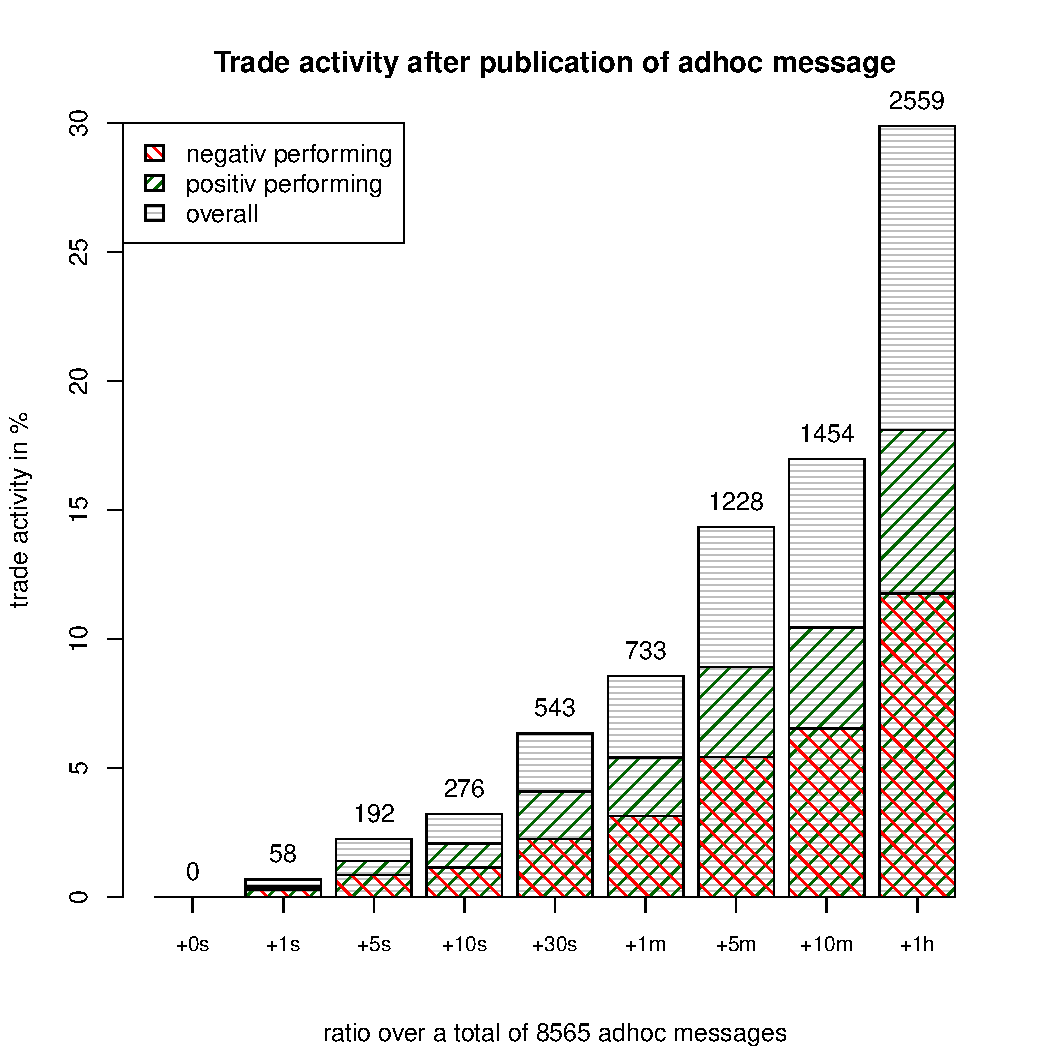
\includegraphics[width=0.70\linewidth]{content/pdf/summary}
\caption{Trade activity after publication of ad~hoc message.}
\label{fig:tradeActivity}
\end{figure}

\Cref{fig:meanPerformance} shows the average stock performance after an ad~hoc message was published. The displayed mean values were calculated from all samples that did show trade activity, \ie the values for '+1s' origin from 58 samples, whereas the values for '+1h' are an aggregation of 2559 values.\\

Nevertheless, since it seems reasonable that within elongating time intervals more trade activity is observed, we can not proof any causality in between the publication of ad~hoc messages and the occurring price fluctuations. In future studies one could analyze preceding points in time as well to compare the trade activity before and after the respective ad~hoc message publication.\\

\begin{figure}[ht!]
\centering
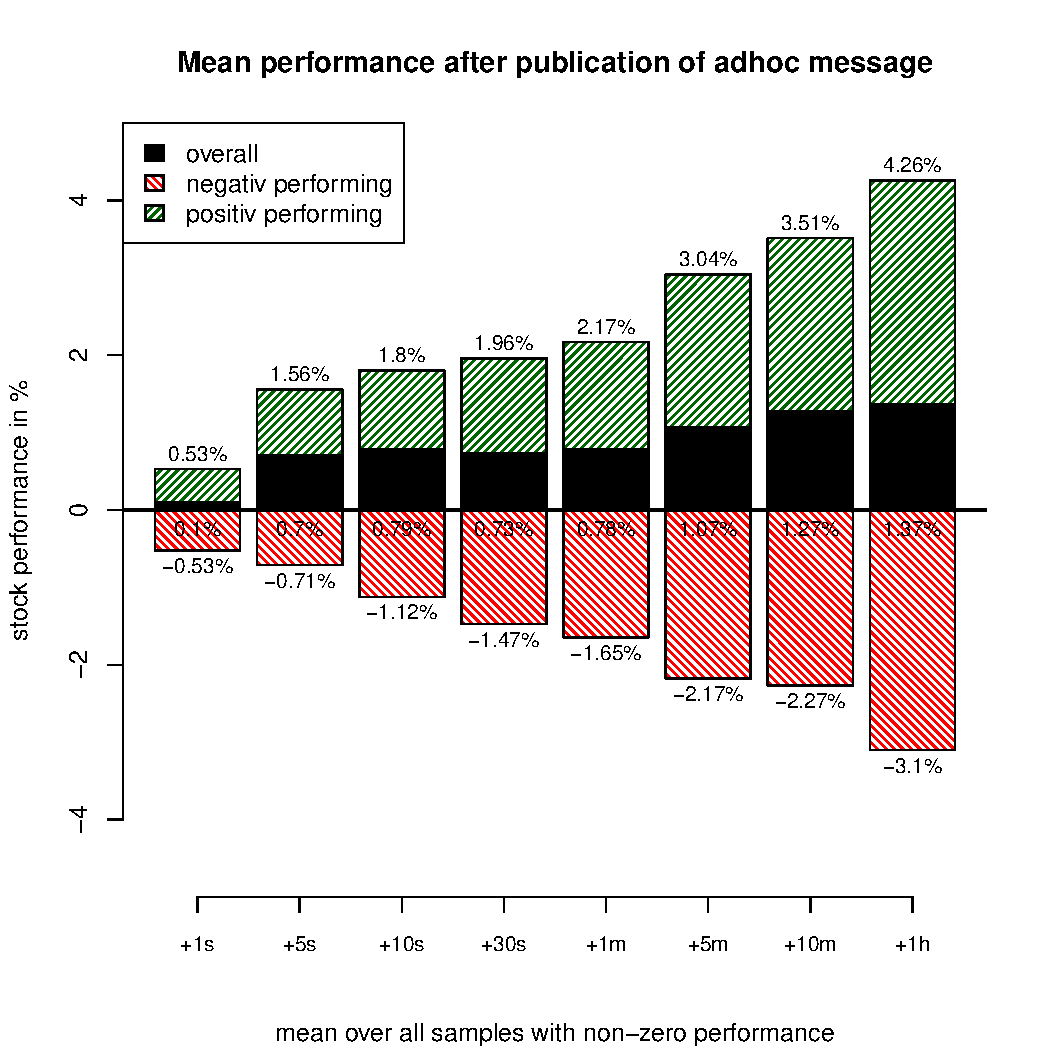
\includegraphics[width=0.70\linewidth]{content/pdf/summary_performance}
\caption{Mean performance after publication of ad~hoc message.}
\label{fig:meanPerformance}
\end{figure}

\chapter{Conclusion}\label{chap:conclusion}
Due to the volume of data, the real world example shown in \Cref{chap:example} would have been a tough job on any single local workstation or students notebook. When analyzing big data, it is a great relief or even an inevitable thing to use a cluster of computer for distributed storage and data processing.\\

Hadoop is a great and powerful cluster framework and R is a highly popular and well-advanced programming language for statisticians. In a world of ever growing data, Hadoop and R make a perfect fit. Both combined, the mightful analytic capabilities of R can be applied to big data.




\eject
 


	\appendix
	%	\pagestyle{scrheadings}
	%	\settocdepth{chapter}
				 
	\backmatter
		\pagestyle{scrheadings}
		\settocdepth{section}
			\input{content/diverse/appendix}
			\clearpage
			
		\pagestyle{empty}
			\chapter{Glossary}
				\begin{acronym}
					\acro{CRAN}{Comprehensive R Archive Network}
					\acro{HDFS}{Hadoop Distributed File System}	
					\acro{GFS}{Google File System}
				\end{acronym}
			\usepackage[                 % !! what about the ``biblatex.cfg''?
        backend=bibtex,      % (bibtex), bibtex8, biber
%        %
        style=numeric-comp,
%        bibstyle=,          % should not be used without citestyle and vice versa
%        citestyle=,
%        natbib=true,
        %
%        sorting=nty,        % (nty), nyt, nyvt, anty, anyt, anyvt, debug, none
%        sortlos=los,        % bib, (los)
%        sortcites=false,    % false
%        maxnames=3,         % <integer> (3)
%        minnames=1,         % (1)
%        maxitems=3,         % (3)
%        minitems=1,         % (1)
%        autocite=,          % inline, footnote, superscript, ...
%        autopunct=true,     % true
%        babel=none,         % (none), hyphen, other, other*
%        block=none,         % (none), space, par, nbpar, ragged
        hyperref=true,      % false
%        backref=false,      % false
%        indexing=false,     % true, (false), cite, bib
%        refsection=none,    % (none), part, chapter, section, subsection
%        refsegment=none,    % (none), part, chapter, section, subsection
%        citereset=none,     % (none), part, chapter, section, subsection
%        abbreviate=true,    % true
%        date=long,          % short, (long)
%        urldate=short,      % (short), long
%        defernums=false,    % false
%        punctfont=false,    % false
        %
%        mincrossrefs=2,     % 2
        bibencoding=inputenc,   % (ascii), inputenc, <encoding>
        %%
%        keywsort=false,     % false
    %
%     useauthor=false,   % true
%     useeditor=false,   % true
%        useprefix=true,     % false
    %
%        pagetracker=true,   % true, (false), page, spread
%     citetracker=true,   % true, (false), context, strict, constrict
%     ibidtracker=true,   % true, (false), context, strict, constrict
%     opcittracker=true,   % true, (false), context, strict, constrict
%     loccittracker=true, % true, (false), context, strict, constrict
%        terseinits=true,    % false
%     labelalpha=true,   % false
%     labelnumber=true,   % false
%     labelyear=true,   % false
%     singletitle=true,   % false
%     uniquename=true,   % true, (false), init
%
        doi=false,
        url=false,
        firstinits=true, % render first/middle names as initals
            ]{biblatex}
            
   \bibliography{bib/literature}
   
      %  \DefineBibliographyStrings{ngerman}{%
         %   bibliography     = {Literaturverzeichnis},  % = \bibname
         %   references       = {Literatur},             % = \refname
     %   }
        \defbibnote{alphabetic}{%
            Die Literaturangaben sind alphabetisch nach den Namen
            der Autoren sortiert. Bei mehreren Autoren wird nach
            dem ersten Autor sortiert.\par
            Und mit dem neuen \LPack{biblatex}-Paket funktioniert
            das auch, wie man unschwer erkennen kann.\par\bigskip
        }


% -------------------------------------------------------------------------------------------------
%% declare author names as "last, first".
%% Either for the first author only or for all authors
%\DeclareNameFormat{author}{%
%    \ifthenelse{\value{listcount}=1}
%        {#1%                                            % first author
%            \ifblank{#3}{}{\addcomma\space #3}}
%        {#1%                                            % all the other authors (last, first)
%            \ifblank{#3}{}{\addcomma\space #3}}%
%%        {\ifblank{#3}{}{#3\space}%                      % all the other authors (first last)
%%            #1}%
%    \ifthenelse{\value{listcount}<\value{liststop}}
%        {,\space}
%            {}
%}
%
%%http://projekte.dante.de/DanteFAQ/BiblatexReihenfolgeAutoren
%\DeclareNameFormat{last-first}{%
%  \iffirstinits
%    {\usebibmacro{name:last-first}{#1}{#4}{#5}{#7}}
%    {\usebibmacro{name:last-first}{#1}{#3}{#5}{#7}}%
%  \usebibmacro{name:andothers}}
%\DeclareNameFormat{labelname}{%
%   \ifuseprefix
%     {\usebibmacro{name:last-first}{#1}{#4}{#5}{#8}}
%     {\usebibmacro{name:last-first}{#1}{#4}{#6}{#8}}%
%   \usebibmacro{name:andothers}}

%  \DefineBibliographyStrings{english}{%
%    typeeditor = {{}{}},
%    typeeditors = {{}{}},
%    in = {{}{}},
%    inseries = {{}{}},
%    byeditor = {{}{}}
%  }

%-------------------------------------------------------------------------------------------------

%% http://www.golatex.de/biblatex-anpassen-die-x-te-frage-t4657.html
\renewbibmacro*{journal+issuetitle}{%
  \usebibmacro{journal}%
  \setunit*{\addcomma\space}%
  \iffieldundef{series}
    {}
    {\newunit
     \printfield{series}%
     \setunit{\addcomma\space}}%
  \printfield{volume}%
  \setunit*{\addcomma\space}%
  \printfield{number}%
  \setunit{\addcomma\space}%
  \printfield{eid}%
  \setunit{\addspace}%
  \usebibmacro{issue+date}%
  \setunit{\addcolon\space}%
  \usebibmacro{issue}%
  \newunit}

\DeclareFieldFormat[article]{volume}{\bibstring{jourvol}~#1}
\DeclareFieldFormat[article]{number}{\bibstring{number}~#1} 
%\DeclareFieldFormat[article]{edition}{\bibstring{edition}~#1} 

%% http://mrunix.de/forums/showthread.php?t=67386
\DefineBibliographyStrings{english}{jourvol={Vol\adddot}} 
\DefineBibliographyStrings{english}{number={No\adddot}} 
\DefineBibliographyStrings{english}{edition={Ed\adddot}} 

\AtBeginBibliography{%
  % Setzt die Autoren-Vornamen auf Kapit�lchen 
  \renewcommand*{\mkbibnamefirst}{\textsc}
  \renewcommand*{\mkbibnamelast}{\textsc}
  \renewcommand*{\mkbibnameprefix}{\textsc}
  \renewcommand*{\mkbibnameaffix}{\textsc}
  
  %%Doppelpunkt nach Namen, kein Punkt
  %\renewcommand*{\labelnamepunct}{\addcolon\space} 
  
  \DeclareFieldFormat{name}{\textsc{#1\isdot}}
  \DeclareFieldFormat{title}{\mkbibemph{#1\isdot}}
  
  %%\DeclareFieldFormat[article]{title}{#1}
  %%\DeclareFieldFormat[article]{title}{\mkbibquote{#1}}
  \renewcommand*{\mkbibquote}[1]{\mkbibemph{#1\isdot}}
 
  % http://tex.stackexchange.com/ ...
  % questions/16716/spell-out-volume-and-edition-in-words-biblatex-in-german
  %\renewcommand*{\mkbibordedition}[1]{\Ordinalstringnum{#1}[f]}
  \renewcommand*{\mkbibordedition}[1]{\ordinalnum{#1}}
}
			\listoffigures 

\listoftables 

\lstlistoflistings
			
\end{document}